\documentclass[11pt]{article}
\usepackage[utf8]{inputenc}
\usepackage[T1]{fontenc}
\usepackage{lmodern}
\usepackage{amsmath,amssymb}
\usepackage[a4paper,margin=2.2cm]{geometry}
\usepackage{graphicx}
\usepackage{float}
\renewcommand{\topfraction}{0.92}
\renewcommand{\bottomfraction}{0.85}
\renewcommand{\textfraction}{0.08}
\renewcommand{\floatpagefraction}{0.75}
\usepackage{booktabs}
\usepackage{tabularx}
\usepackage{array}
\usepackage{enumitem}
\usepackage{microtype}
\usepackage{titlesec}
\usepackage{caption}
\usepackage[dvipsnames]{xcolor}
\usepackage{cite}
\usepackage[colorlinks=true,allcolors=Blue,breaklinks=true]{hyperref}
\usepackage{pgfplots}
\pgfplotsset{compat=1.18}
\usepgfplotslibrary{fillbetween}
\usepgfplotslibrary{groupplots}
\usetikzlibrary{arrows.meta,positioning,backgrounds,fit,calc}
\definecolor{oiBlue}{HTML}{0072B2}
\definecolor{oiOrange}{HTML}{E69F00}
\definecolor{oiGreen}{HTML}{009E73}
\definecolor{oiVerm}{HTML}{D55E00}
\definecolor{oiPurple}{HTML}{8256B4}
\definecolor{oiSky}{HTML}{56B4E9}
\definecolor{oiGrey}{HTML}{8A8A8A}
\definecolor{oiInk}{HTML}{222222}
\pgfplotsset{
  paperplot/.style={
    axis line style={oiInk!75, line width=0.5pt},
    tick label style={font=\small}, label style={font=\small},
    title style={font=\small, align=center},
    grid=major, grid style={oiInk!12, line width=0.4pt},
    tick align=outside, tickpos=left, axis on top=false,
    legend style={font=\footnotesize, draw=none, fill=none, row sep=1pt},
    legend cell align=left,
  }
}

\captionsetup{font=small,labelfont=bf,labelsep=period}
\titleformat{\section}{\normalfont\large\bfseries}{\thesection.}{0.6em}{}
\titleformat{\subsection}{\normalfont\normalsize\bfseries}{\thesubsection}{0.6em}{}
\newcommand{\ent}[1]{\raisebox{0.1ex}{\textcircled{\scriptsize #1}}}
\setlength{\parskip}{0.35em}
\setlength{\parindent}{0pt}
\frenchspacing
\sloppy
\hyphenpenalty=1200
\title{\vspace{-1.2cm}\bfseries Machine learning for sample-based quantum diagonalization: generative configuration recovery and the classical-simulability frontier}
\author{Nicol\'as Bonilla Vargas\thanks{M.Sc.\ Physics, Universidad Nacional de Colombia; M.Sc.\ Applied Data Science \& AI, SRH University Heidelberg / Munich. \texttt{ngbonillav@unal.edu.co}}}
\date{\today}

\begin{document}
\maketitle
\begin{abstract}
Sample-based quantum diagonalization (SQD), equivalently quantum-selected configuration interaction (QSCI), has in two years become the pragmatic centre of gravity of pre-fault-tolerant quantum chemistry: a quantum processor samples electronic configurations, and the many-electron Hamiltonian is diagonalized classically in the resulting determinant subspace. Its accuracy is governed entirely by \emph{which} configurations enter that subspace, a selection problem for machine learning, made acute by a coupon-collector bottleneck. We critically review the resulting ecosystem of generative and learned selectors, organizing it by the object each method generates and the importance signal it exploits, and expose one conspicuous gap: a reward-proportional generative-flow-network proposer built for tail discovery itself. We then confront the field's central question --- whether the quantum sampler beats classical selected configuration interaction --- and report a carefully scoped negative: across the published same-active-space comparisons, strong classical selected CI matches or beats the quantum-sampled subspace, and the flagship single-layer circuits now admit polynomial-time classical energy estimation. We distil a benchmarking standard and turn the negative into a regime map --- a quantum or generative edge can survive only where the classical heuristic that makes an SQD subspace \emph{verifiable} also fails to \emph{construct} it cheaply --- then test it with FCI-exact experiments that confirm one prediction and refute another: the cheap prior's rank correlation with the exact weights declines with multireference character (a usable coordinate), but a controlled single-molecule noise sweep shows the one generative advantage we find, robustness to valid-shot starvation, to be generic rather than the multireference-specific effect a confounded contrast first suggested. Finally, we flag learning from quantum experiments, whose classical sample-complexity lower bound is an unconditional theorem, as the one adjacent frontier where a quantum advantage is provable but its bridge to chemistry remains unbuilt.
\end{abstract}

\section{Introduction}\label{sec:1}

The determination of the ground-state energy of a many-electron Hamiltonian is among the oldest and most consequential problems in the physical sciences, underlying our predictive understanding of chemical reactivity, catalysis, and correlated materials. Its difficulty is structural: the dimension of the full configuration-interaction (FCI) space grows combinatorially with the number of electrons and orbitals, and the exact problem is, in the worst case, QMA-complete \cite{kempe2006}. The last half-century of quantum chemistry can be read as a sequence of increasingly sophisticated strategies for evading this exponential wall without paying its full cost --- coupled-cluster expansions, the density-matrix renormalization group (DMRG), auxiliary-field quantum Monte Carlo (AFQMC), and, most directly relevant here, \emph{selected} configuration interaction (sCI), which builds a compact variational subspace by retaining only the determinants that matter and correcting the remainder perturbatively \cite{huron1973,holmes2016,sharma2017,tubman2016}.

The advent of programmable quantum processors reframed the same problem. If the exponential difficulty of electronic structure is a quantum difficulty, perhaps a quantum device can help. The first decade of this hope was dominated by the variational quantum eigensolver (VQE) \cite{peruzzo2014}, in which a parameterized circuit is optimized to minimize an energy expectation value. That programme has, for the purpose of demonstrating a scaling advantage, largely run its course: barren plateaus render deep expressive circuits untrainable \cite{mcclean2018,larocca2025}, the measurement cost of estimating chemical-accuracy energies is prohibitive, and --- most damningly --- the structural conditions that let a variational circuit \emph{avoid} barren plateaus tend also to render it classically simulable \cite{cerezo2025}. Into the vacuum left by VQE stepped a conceptually different, and strikingly effective, idea.

\textbf{Sample-based quantum diagonalization.} Rather than optimize a circuit to \emph{be} the ground state, one uses a shallow, noise-tolerant circuit only to \emph{sample} the electronic configurations (computational-basis bitstrings, i.e.\ Slater determinants) that carry appreciable ground-state weight, and then diagonalizes the Hamiltonian classically in the sampled subspace on high-performance hardware. Introduced as quantum-selected configuration interaction (QSCI) by Kanno and co-workers \cite{kanno2023} and scaled to quantum-centric supercomputing as SQD by an IBM--RIKEN collaboration \cite{robledomoreno2025}, the method inherits the variational guarantee of sCI, sidesteps the optimization and measurement pathologies of VQE, and is remarkably robust to hardware noise through a self-consistent configuration-recovery step that repairs symmetry-broken samples. Within two years it has been demonstrated on iron--sulfur clusters at 77 qubits with the entire Fugaku supercomputer in the loop \cite{robledomoreno2025,shirakawa2025}, extended to excited states, embeddings, and periodic systems, and pushed, through fragment-based workflows, to a 12,635-atom protein--ligand complex \cite{wang2026}. SQD is, today, the de facto default of pre-fault-tolerant quantum chemistry.

\textbf{The machine-learning entry point.} The accuracy of the SQD loop is determined entirely by which configurations populate the subspace, and this is where the method is most vulnerable and most interesting. The relevant determinants are heavy-tailed in amplitude; discovering the rare, chemically decisive ones by repeated sampling is a coupon-collector problem, in which the marginal cost of each newly discovered configuration grows sharply \cite{reinholdt2025}. The configuration-recovery step, a probabilistic repair of noise-corrupted samples toward an estimated occupation profile, is a statistical denoising problem. Both are natural targets for machine learning, and the field has responded with striking speed. In the two years since QSCI, generative and learned methods have been proposed for every stage of the loop: restricted Boltzmann machines that learn and resample the distribution of dominant determinants \cite{patra2025,patra2026}; autoregressive and transformer neural quantum states that propose determinants inside the sample--diagonalize--update loop \cite{chang2026,solanki2026,shang2025}; neural-network classifiers and learning-to-rank models that predict determinant importance \cite{zeni2026,zhanghaar2025,nie2026}; and generative circuit design that learns the sampling ansatz itself \cite{kemmoku2026}. This ecosystem has, to our knowledge, never been reviewed, and it is growing faster than any single group can track.

\textbf{The question the field turns on.} Beneath the methodological activity lies a single, contested, and increasingly uncomfortable question: does any of this actually beat classical selected configuration interaction? SQD \emph{is}, after all, a quantum-sampled sCI, and its classical competitors --- semistochastic heat-bath CI (SHCI), the perturbatively-selected CIPSI, adaptive sampling CI (ASCI), DMRG, and AFQMC --- are mature, fast, and run on a laptop. The critical literature has grown in tandem with the method. Reinholdt and co-workers showed that, even granting SQD a perfect noiseless sampler, its expansions are an order of magnitude less compact than heat-bath CI on the very systems used to showcase it \cite{reinholdt2025}; Gaberle and Jattana found that for strongly correlated lattice models the required configuration count grows exponentially \emph{even with an optimal sampler} \cite{gaberle2026}; Vaquero-Sabater and co-workers demonstrated that random determinants passed through the classical recovery loop reproduce the accuracy, implying that the classical recovery, not the quantum sampler, is doing the work \cite{vaquerosabater2026}; and, most strikingly, Belagali and co-workers showed in 2026 that the single-layer local unitary cluster Jastrow circuit SQD samples is classically simulable in polynomial time, reproducing the flagship 77-qubit experiment on a laptop at \emph{lower} energy --- at the energy (weak-simulation) level, not by out-sampling the device \cite{belagali2026}. The pro-quantum case remains alive but narrow: worst-case instantaneous-quantum-polynomial (IQP) hardness of the sampling circuits \cite{hafid2025}, and a contested 49-qubit advantage claim on sparse-ground-state Hamiltonians \cite{kirby2026}.

\textbf{This review.} We take the position that a field cannot mature while its central claim is unsettled, and that the right place to stand is neither uncritical enthusiasm nor dismissal, but a rigorous map of what is known. We make five contributions. First (\S\ref{sec:2}--\S\ref{sec:3}), we give a structured account of the SQD/QSCI method family and the configuration-recovery bottleneck that makes it a machine-learning problem. Second (\S\ref{sec:4}), we provide the first taxonomy of the ML and generative methods proposed for determinant and subspace selection, organized by the object they generate and the importance signal they exploit, and we identify the conspicuous methodological gap: that generative flow networks, purpose-built for diverse reward-proportional sampling over exponential discrete spaces, have not yet been applied to this problem. Third (\S\ref{sec:5}), we confront the quantum-advantage question directly, assembling the classical baselines, the benzene-benchmark accuracy standard, the critique literature, and the 2026 dequantization results into a single defensible verdict. Fourth (\S\ref{sec:6}), we propose a set of benchmarking standards that we contend any future claim in this field must meet. Fifth (\S\ref{sec:7}), we argue that the negative result is a compass, identifying where generative and quantum methods might retain a defensible or, in one case, provable advantage: robustness under device noise (which a controlled test finds to be generic rather than a quantum edge), genuinely multireference chemistry (an open prediction we probe but do not confirm), and the distinct quantum-data-native task of learning from experiments. Throughout, we distinguish sharply between what is proven, what is demonstrated, and what is hoped.

\medskip\noindent\textbf{Abbreviations.} {\footnotesize SQD/QSCI (sample-based quantum diagonalization / quantum-selected configuration interaction); sCI (selected configuration interaction); SHCI (semistochastic heat-bath CI); CIPSI (perturbatively selected CI); ASCI (adaptive sampling CI); FCI (full configuration interaction); DMRG (density-matrix renormalization group); AFQMC (auxiliary-field quantum Monte Carlo); LUCJ (local unitary cluster Jastrow); S-CORE (self-consistent configuration recovery); VQE (variational quantum eigensolver); NQS (neural quantum state); RBM (restricted Boltzmann machine); GQE (generative quantum eigensolver); GFlowNet (generative flow network); EN (Epstein--Nesbet); PT (perturbation theory).}


\section{Sample-based quantum diagonalization: the method and its family}\label{sec:2}

\emph{Scope and method.} This review surveys the sample-based quantum diagonalization literature indexed on arXiv (quant-ph, physics.chem-ph) and in the major chemistry and quantum-information journals, together with the community bibliography \emph{Awesome-QSCI}, from the introduction of QSCI in early 2023 to mid-2026. We include the SQD/QSCI method family, the machine-learning and generative methods proposed for determinant or subspace selection, the classical selected-configuration-interaction competitors that constitute the benchmark, and the critique and dequantization literature; we exclude general variational-quantum-eigensolver work except where it bears directly on the sampling step. Because the field is moving on a scale of weeks and much of the primary literature is preprint, we date every claim explicitly and flag its standing --- established, demonstrated, or merely hoped.


\subsection{The core loop}\label{sec:2-1}


\begin{figure*}[tb]
\centering
\resizebox{\linewidth}{!}{%
\begin{tikzpicture}[font=\sffamily,every node/.style={inner sep=0pt}]
\fill[oiSky!8,rounded corners=8pt] (0,4.7) rectangle (17.4,9.5);
\draw[oiBlue!45,line width=1pt,rounded corners=8pt] (0,4.7) rectangle (17.4,9.5);
\fill[oiPurple!6,rounded corners=8pt] (0,-1.3) rectangle (17.4,3.5);
\draw[oiPurple!45,line width=1pt,rounded corners=8pt] (0,-1.3) rectangle (17.4,3.5);
\node[anchor=north,font=\small\bfseries,text=oiBlue] at (8.70,9.35) {QUANTUM PROCESSOR};
\node[anchor=south,font=\small\bfseries,text=oiPurple] at (8.70,-1.15) {CLASSICAL CO-PROCESSOR (HPC)};
\node[anchor=north,font=\footnotesize\bfseries,text=oiInk] at (2.75,8.85) {1 $\cdot$ Molecule + Hamiltonian};
\node[anchor=north,font=\footnotesize\bfseries,text=oiInk] at (8.70,8.85) {2 $\cdot$ LUCJ circuit on QPU};
\node[anchor=north,font=\footnotesize\bfseries,text=oiInk] at (14.65,8.85) {3 $\cdot$ Sample bitstrings};
\node[anchor=center] at (2.75,6.7) {\begin{tikzpicture}\draw[oiInk!40,line width=2pt] (-0.45,0)--(0.45,0);\fill[oiBlue] (-0.45,0) circle (5pt);\fill[oiBlue] (0.45,0) circle (5pt);\node[font=\tiny,text=oiInk!70,anchor=north] at (0,-0.28){N$_2$, $R=2.0$\,\AA};\end{tikzpicture}};
\node[anchor=north,font=\tiny,text=oiInk!60] at (2.75,4.98) {CAS(10e, 12o), exact-FCI-verifiable};
\node[anchor=center] at (8.70,6.55) {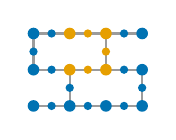
\begin{tikzpicture}\draw[oiInk!45,line width=0.8pt] (0.00,0.00)--(1.38,0.00);\draw[oiInk!45,line width=0.8pt] (0.00,0.46)--(1.38,0.46);\draw[oiInk!45,line width=0.8pt] (0.00,0.92)--(1.38,0.92);\draw[oiInk!45,line width=0.8pt] (0.00,0.92)--(0.00,0.46);\draw[oiInk!45,line width=0.8pt] (0.92,0.92)--(0.92,0.46);\draw[oiInk!45,line width=0.8pt] (0.46,0.46)--(0.46,0.00);\draw[oiInk!45,line width=0.8pt] (1.38,0.46)--(1.38,0.00);\fill[oiBlue] (0.00,0.00) circle (2.1pt);\fill[oiBlue] (0.46,0.00) circle (2.1pt);\fill[oiBlue] (0.92,0.00) circle (2.1pt);\fill[oiBlue] (1.38,0.00) circle (2.1pt);\fill[oiBlue] (0.00,0.46) circle (2.1pt);\fill[oiOrange] (0.46,0.46) circle (2.1pt);\fill[oiOrange] (0.92,0.46) circle (2.1pt);\fill[oiBlue] (1.38,0.46) circle (2.1pt);\fill[oiBlue] (0.00,0.92) circle (2.1pt);\fill[oiOrange] (0.46,0.92) circle (2.1pt);\fill[oiOrange] (0.92,0.92) circle (2.1pt);\fill[oiBlue] (1.38,0.92) circle (2.1pt);\fill[oiBlue] (0.23,0.00) circle (1.5pt);\fill[oiBlue] (0.69,0.00) circle (1.5pt);\fill[oiBlue] (1.15,0.00) circle (1.5pt);\fill[oiBlue] (0.23,0.46) circle (1.5pt);\fill[oiOrange] (0.69,0.46) circle (1.5pt);\fill[oiBlue] (1.15,0.46) circle (1.5pt);\fill[oiBlue] (0.23,0.92) circle (1.5pt);\fill[oiOrange] (0.69,0.92) circle (1.5pt);\fill[oiBlue] (1.15,0.92) circle (1.5pt);\fill[oiBlue] (0.00,0.69) circle (1.5pt);\fill[oiOrange] (0.92,0.69) circle (1.5pt);\fill[oiBlue] (0.46,0.23) circle (1.5pt);\fill[oiBlue] (1.38,0.23) circle (1.5pt);\end{tikzpicture}};
\node[anchor=north,font=\tiny,text=oiOrange!85!black] at (8.70,4.98) {heavy-hex qubits $\cdot$ LUCJ patch (orange)};
\node[anchor=center] at (14.65,6.75) {\begin{tikzpicture}\begin{axis}[width=3.15cm,height=2.35cm,scale only axis,grid=none,axis line style={oiInk!55,line width=0.5pt},tick align=outside,tick label style={font=\tiny,text=oiInk!80},label style={font=\tiny,text=oiInk},tickpos=left,every axis plot/.append style={line width=0.9pt},xbar,y dir=reverse,bar width=2.4pt,xmin=0,xmax=1200,ymin=-0.7,ymax=13.7,axis y line=none,axis x line=bottom,xlabel={counts},xtick distance=600,enlarge y limits=false]\addplot[fill=oiBlue,draw=none] table[x=count,y=rank]{wf_hist.dat};\end{axis}\end{tikzpicture}};
\node[anchor=north,font=\tiny,text=oiInk!60,align=center] at (14.65,4.98) {$\sim$77\% valid shots (Heron noise)};
\draw[-{Stealth[length=2.4mm]},oiInk!65,line width=1pt] (4.25,6.7)--(6.80,6.7);
\draw[-{Stealth[length=2.4mm]},oiInk!65,line width=1pt] (10.60,6.7)--(12.75,6.7);
\node[anchor=north,font=\footnotesize\bfseries,text=oiInk] at (2.75,2.9) {6 $\cdot$ Diagonalize $\rightarrow E_0$};
\node[anchor=north,font=\footnotesize\bfseries,text=oiInk] at (8.70,2.9) {5 $\cdot$ Determinant subspace $\mathcal{S}$};
\node[anchor=north,font=\footnotesize\bfseries,text=oiInk] at (14.65,2.9) {4 $\cdot$ S-CORE recovery};
\node[anchor=center] at (14.65,0.75) {\begin{tikzpicture}\begin{axis}[width=3.15cm,height=2.35cm,scale only axis,grid=none,axis line style={oiInk!55,line width=0.5pt},tick align=outside,tick label style={font=\tiny,text=oiInk!80},label style={font=\tiny,text=oiInk},tickpos=left,every axis plot/.append style={line width=0.9pt},ybar,bar width=2.0pt,xmin=-0.8,xmax=11.8,ymin=0,ymax=1.05,xlabel={orbital $p$},ylabel={$\langle n_p\rangle$},xtick={0,5,10},ytick={0,0.5,1}]\addplot[fill=oiPurple,draw=none] table[x=orb,y=occ]{wf_occ.dat};\draw[oiVerm,densely dashed,line width=0.6pt] (axis cs:-0.8,0.417)--(axis cs:11.8,0.417);\end{axis}\end{tikzpicture}};
\node[anchor=north] at (8.70,2.60) {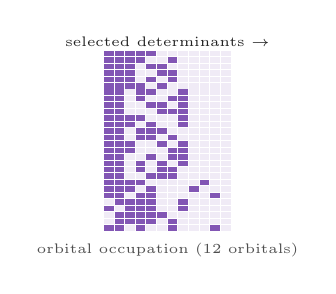
\begin{tikzpicture}\node[anchor=north,font=\tiny,text=oiInk] at (0.81,0.30) {selected determinants $\rightarrow$};\fill[oiPurple] (0.000,0.000) rectangle (0.123,-0.070);\fill[oiPurple] (0.135,0.000) rectangle (0.258,-0.070);\fill[oiPurple] (0.270,0.000) rectangle (0.393,-0.070);\fill[oiPurple] (0.405,0.000) rectangle (0.528,-0.070);\fill[oiPurple] (0.540,0.000) rectangle (0.663,-0.070);\fill[oiPurple!12] (0.675,0.000) rectangle (0.798,-0.070);\fill[oiPurple!12] (0.810,0.000) rectangle (0.933,-0.070);\fill[oiPurple!12] (0.945,0.000) rectangle (1.068,-0.070);\fill[oiPurple!12] (1.080,0.000) rectangle (1.203,-0.070);\fill[oiPurple!12] (1.215,0.000) rectangle (1.338,-0.070);\fill[oiPurple!12] (1.350,0.000) rectangle (1.473,-0.070);\fill[oiPurple!12] (1.485,0.000) rectangle (1.608,-0.070);\fill[oiPurple] (0.000,-0.082) rectangle (0.123,-0.152);\fill[oiPurple] (0.135,-0.082) rectangle (0.258,-0.152);\fill[oiPurple] (0.270,-0.082) rectangle (0.393,-0.152);\fill[oiPurple] (0.405,-0.082) rectangle (0.528,-0.152);\fill[oiPurple!12] (0.540,-0.082) rectangle (0.663,-0.152);\fill[oiPurple!12] (0.675,-0.082) rectangle (0.798,-0.152);\fill[oiPurple] (0.810,-0.082) rectangle (0.933,-0.152);\fill[oiPurple!12] (0.945,-0.082) rectangle (1.068,-0.152);\fill[oiPurple!12] (1.080,-0.082) rectangle (1.203,-0.152);\fill[oiPurple!12] (1.215,-0.082) rectangle (1.338,-0.152);\fill[oiPurple!12] (1.350,-0.082) rectangle (1.473,-0.152);\fill[oiPurple!12] (1.485,-0.082) rectangle (1.608,-0.152);\fill[oiPurple] (0.000,-0.164) rectangle (0.123,-0.234);\fill[oiPurple] (0.135,-0.164) rectangle (0.258,-0.234);\fill[oiPurple] (0.270,-0.164) rectangle (0.393,-0.234);\fill[oiPurple!12] (0.405,-0.164) rectangle (0.528,-0.234);\fill[oiPurple] (0.540,-0.164) rectangle (0.663,-0.234);\fill[oiPurple] (0.675,-0.164) rectangle (0.798,-0.234);\fill[oiPurple!12] (0.810,-0.164) rectangle (0.933,-0.234);\fill[oiPurple!12] (0.945,-0.164) rectangle (1.068,-0.234);\fill[oiPurple!12] (1.080,-0.164) rectangle (1.203,-0.234);\fill[oiPurple!12] (1.215,-0.164) rectangle (1.338,-0.234);\fill[oiPurple!12] (1.350,-0.164) rectangle (1.473,-0.234);\fill[oiPurple!12] (1.485,-0.164) rectangle (1.608,-0.234);\fill[oiPurple] (0.000,-0.246) rectangle (0.123,-0.316);\fill[oiPurple] (0.135,-0.246) rectangle (0.258,-0.316);\fill[oiPurple] (0.270,-0.246) rectangle (0.393,-0.316);\fill[oiPurple!12] (0.405,-0.246) rectangle (0.528,-0.316);\fill[oiPurple!12] (0.540,-0.246) rectangle (0.663,-0.316);\fill[oiPurple] (0.675,-0.246) rectangle (0.798,-0.316);\fill[oiPurple] (0.810,-0.246) rectangle (0.933,-0.316);\fill[oiPurple!12] (0.945,-0.246) rectangle (1.068,-0.316);\fill[oiPurple!12] (1.080,-0.246) rectangle (1.203,-0.316);\fill[oiPurple!12] (1.215,-0.246) rectangle (1.338,-0.316);\fill[oiPurple!12] (1.350,-0.246) rectangle (1.473,-0.316);\fill[oiPurple!12] (1.485,-0.246) rectangle (1.608,-0.316);\fill[oiPurple] (0.000,-0.328) rectangle (0.123,-0.398);\fill[oiPurple] (0.135,-0.328) rectangle (0.258,-0.398);\fill[oiPurple] (0.270,-0.328) rectangle (0.393,-0.398);\fill[oiPurple!12] (0.405,-0.328) rectangle (0.528,-0.398);\fill[oiPurple] (0.540,-0.328) rectangle (0.663,-0.398);\fill[oiPurple!12] (0.675,-0.328) rectangle (0.798,-0.398);\fill[oiPurple] (0.810,-0.328) rectangle (0.933,-0.398);\fill[oiPurple!12] (0.945,-0.328) rectangle (1.068,-0.398);\fill[oiPurple!12] (1.080,-0.328) rectangle (1.203,-0.398);\fill[oiPurple!12] (1.215,-0.328) rectangle (1.338,-0.398);\fill[oiPurple!12] (1.350,-0.328) rectangle (1.473,-0.398);\fill[oiPurple!12] (1.485,-0.328) rectangle (1.608,-0.398);\fill[oiPurple] (0.000,-0.410) rectangle (0.123,-0.480);\fill[oiPurple] (0.135,-0.410) rectangle (0.258,-0.480);\fill[oiPurple] (0.270,-0.410) rectangle (0.393,-0.480);\fill[oiPurple] (0.405,-0.410) rectangle (0.528,-0.480);\fill[oiPurple!12] (0.540,-0.410) rectangle (0.663,-0.480);\fill[oiPurple] (0.675,-0.410) rectangle (0.798,-0.480);\fill[oiPurple!12] (0.810,-0.410) rectangle (0.933,-0.480);\fill[oiPurple!12] (0.945,-0.410) rectangle (1.068,-0.480);\fill[oiPurple!12] (1.080,-0.410) rectangle (1.203,-0.480);\fill[oiPurple!12] (1.215,-0.410) rectangle (1.338,-0.480);\fill[oiPurple!12] (1.350,-0.410) rectangle (1.473,-0.480);\fill[oiPurple!12] (1.485,-0.410) rectangle (1.608,-0.480);\fill[oiPurple] (0.000,-0.492) rectangle (0.123,-0.562);\fill[oiPurple] (0.135,-0.492) rectangle (0.258,-0.562);\fill[oiPurple!12] (0.270,-0.492) rectangle (0.393,-0.562);\fill[oiPurple] (0.405,-0.492) rectangle (0.528,-0.562);\fill[oiPurple] (0.540,-0.492) rectangle (0.663,-0.562);\fill[oiPurple!12] (0.675,-0.492) rectangle (0.798,-0.562);\fill[oiPurple!12] (0.810,-0.492) rectangle (0.933,-0.562);\fill[oiPurple] (0.945,-0.492) rectangle (1.068,-0.562);\fill[oiPurple!12] (1.080,-0.492) rectangle (1.203,-0.562);\fill[oiPurple!12] (1.215,-0.492) rectangle (1.338,-0.562);\fill[oiPurple!12] (1.350,-0.492) rectangle (1.473,-0.562);\fill[oiPurple!12] (1.485,-0.492) rectangle (1.608,-0.562);\fill[oiPurple] (0.000,-0.574) rectangle (0.123,-0.644);\fill[oiPurple] (0.135,-0.574) rectangle (0.258,-0.644);\fill[oiPurple!12] (0.270,-0.574) rectangle (0.393,-0.644);\fill[oiPurple] (0.405,-0.574) rectangle (0.528,-0.644);\fill[oiPurple!12] (0.540,-0.574) rectangle (0.663,-0.644);\fill[oiPurple!12] (0.675,-0.574) rectangle (0.798,-0.644);\fill[oiPurple] (0.810,-0.574) rectangle (0.933,-0.644);\fill[oiPurple] (0.945,-0.574) rectangle (1.068,-0.644);\fill[oiPurple!12] (1.080,-0.574) rectangle (1.203,-0.644);\fill[oiPurple!12] (1.215,-0.574) rectangle (1.338,-0.644);\fill[oiPurple!12] (1.350,-0.574) rectangle (1.473,-0.644);\fill[oiPurple!12] (1.485,-0.574) rectangle (1.608,-0.644);\fill[oiPurple] (0.000,-0.656) rectangle (0.123,-0.726);\fill[oiPurple] (0.135,-0.656) rectangle (0.258,-0.726);\fill[oiPurple!12] (0.270,-0.656) rectangle (0.393,-0.726);\fill[oiPurple!12] (0.405,-0.656) rectangle (0.528,-0.726);\fill[oiPurple] (0.540,-0.656) rectangle (0.663,-0.726);\fill[oiPurple] (0.675,-0.656) rectangle (0.798,-0.726);\fill[oiPurple!12] (0.810,-0.656) rectangle (0.933,-0.726);\fill[oiPurple] (0.945,-0.656) rectangle (1.068,-0.726);\fill[oiPurple!12] (1.080,-0.656) rectangle (1.203,-0.726);\fill[oiPurple!12] (1.215,-0.656) rectangle (1.338,-0.726);\fill[oiPurple!12] (1.350,-0.656) rectangle (1.473,-0.726);\fill[oiPurple!12] (1.485,-0.656) rectangle (1.608,-0.726);\fill[oiPurple] (0.000,-0.738) rectangle (0.123,-0.808);\fill[oiPurple] (0.135,-0.738) rectangle (0.258,-0.808);\fill[oiPurple!12] (0.270,-0.738) rectangle (0.393,-0.808);\fill[oiPurple!12] (0.405,-0.738) rectangle (0.528,-0.808);\fill[oiPurple!12] (0.540,-0.738) rectangle (0.663,-0.808);\fill[oiPurple] (0.675,-0.738) rectangle (0.798,-0.808);\fill[oiPurple] (0.810,-0.738) rectangle (0.933,-0.808);\fill[oiPurple] (0.945,-0.738) rectangle (1.068,-0.808);\fill[oiPurple!12] (1.080,-0.738) rectangle (1.203,-0.808);\fill[oiPurple!12] (1.215,-0.738) rectangle (1.338,-0.808);\fill[oiPurple!12] (1.350,-0.738) rectangle (1.473,-0.808);\fill[oiPurple!12] (1.485,-0.738) rectangle (1.608,-0.808);\fill[oiPurple] (0.000,-0.820) rectangle (0.123,-0.890);\fill[oiPurple] (0.135,-0.820) rectangle (0.258,-0.890);\fill[oiPurple] (0.270,-0.820) rectangle (0.393,-0.890);\fill[oiPurple] (0.405,-0.820) rectangle (0.528,-0.890);\fill[oiPurple!12] (0.540,-0.820) rectangle (0.663,-0.890);\fill[oiPurple!12] (0.675,-0.820) rectangle (0.798,-0.890);\fill[oiPurple!12] (0.810,-0.820) rectangle (0.933,-0.890);\fill[oiPurple] (0.945,-0.820) rectangle (1.068,-0.890);\fill[oiPurple!12] (1.080,-0.820) rectangle (1.203,-0.890);\fill[oiPurple!12] (1.215,-0.820) rectangle (1.338,-0.890);\fill[oiPurple!12] (1.350,-0.820) rectangle (1.473,-0.890);\fill[oiPurple!12] (1.485,-0.820) rectangle (1.608,-0.890);\fill[oiPurple] (0.000,-0.902) rectangle (0.123,-0.972);\fill[oiPurple] (0.135,-0.902) rectangle (0.258,-0.972);\fill[oiPurple] (0.270,-0.902) rectangle (0.393,-0.972);\fill[oiPurple!12] (0.405,-0.902) rectangle (0.528,-0.972);\fill[oiPurple] (0.540,-0.902) rectangle (0.663,-0.972);\fill[oiPurple!12] (0.675,-0.902) rectangle (0.798,-0.972);\fill[oiPurple!12] (0.810,-0.902) rectangle (0.933,-0.972);\fill[oiPurple] (0.945,-0.902) rectangle (1.068,-0.972);\fill[oiPurple!12] (1.080,-0.902) rectangle (1.203,-0.972);\fill[oiPurple!12] (1.215,-0.902) rectangle (1.338,-0.972);\fill[oiPurple!12] (1.350,-0.902) rectangle (1.473,-0.972);\fill[oiPurple!12] (1.485,-0.902) rectangle (1.608,-0.972);\fill[oiPurple] (0.000,-0.984) rectangle (0.123,-1.054);\fill[oiPurple] (0.135,-0.984) rectangle (0.258,-1.054);\fill[oiPurple!12] (0.270,-0.984) rectangle (0.393,-1.054);\fill[oiPurple] (0.405,-0.984) rectangle (0.528,-1.054);\fill[oiPurple] (0.540,-0.984) rectangle (0.663,-1.054);\fill[oiPurple] (0.675,-0.984) rectangle (0.798,-1.054);\fill[oiPurple!12] (0.810,-0.984) rectangle (0.933,-1.054);\fill[oiPurple!12] (0.945,-0.984) rectangle (1.068,-1.054);\fill[oiPurple!12] (1.080,-0.984) rectangle (1.203,-1.054);\fill[oiPurple!12] (1.215,-0.984) rectangle (1.338,-1.054);\fill[oiPurple!12] (1.350,-0.984) rectangle (1.473,-1.054);\fill[oiPurple!12] (1.485,-0.984) rectangle (1.608,-1.054);\fill[oiPurple] (0.000,-1.066) rectangle (0.123,-1.136);\fill[oiPurple] (0.135,-1.066) rectangle (0.258,-1.136);\fill[oiPurple!12] (0.270,-1.066) rectangle (0.393,-1.136);\fill[oiPurple] (0.405,-1.066) rectangle (0.528,-1.136);\fill[oiPurple] (0.540,-1.066) rectangle (0.663,-1.136);\fill[oiPurple!12] (0.675,-1.066) rectangle (0.798,-1.136);\fill[oiPurple] (0.810,-1.066) rectangle (0.933,-1.136);\fill[oiPurple!12] (0.945,-1.066) rectangle (1.068,-1.136);\fill[oiPurple!12] (1.080,-1.066) rectangle (1.203,-1.136);\fill[oiPurple!12] (1.215,-1.066) rectangle (1.338,-1.136);\fill[oiPurple!12] (1.350,-1.066) rectangle (1.473,-1.136);\fill[oiPurple!12] (1.485,-1.066) rectangle (1.608,-1.136);\fill[oiPurple] (0.000,-1.148) rectangle (0.123,-1.218);\fill[oiPurple] (0.135,-1.148) rectangle (0.258,-1.218);\fill[oiPurple] (0.270,-1.148) rectangle (0.393,-1.218);\fill[oiPurple!12] (0.405,-1.148) rectangle (0.528,-1.218);\fill[oiPurple!12] (0.540,-1.148) rectangle (0.663,-1.218);\fill[oiPurple] (0.675,-1.148) rectangle (0.798,-1.218);\fill[oiPurple!12] (0.810,-1.148) rectangle (0.933,-1.218);\fill[oiPurple] (0.945,-1.148) rectangle (1.068,-1.218);\fill[oiPurple!12] (1.080,-1.148) rectangle (1.203,-1.218);\fill[oiPurple!12] (1.215,-1.148) rectangle (1.338,-1.218);\fill[oiPurple!12] (1.350,-1.148) rectangle (1.473,-1.218);\fill[oiPurple!12] (1.485,-1.148) rectangle (1.608,-1.218);\fill[oiPurple] (0.000,-1.230) rectangle (0.123,-1.300);\fill[oiPurple] (0.135,-1.230) rectangle (0.258,-1.300);\fill[oiPurple] (0.270,-1.230) rectangle (0.393,-1.300);\fill[oiPurple!12] (0.405,-1.230) rectangle (0.528,-1.300);\fill[oiPurple!12] (0.540,-1.230) rectangle (0.663,-1.300);\fill[oiPurple!12] (0.675,-1.230) rectangle (0.798,-1.300);\fill[oiPurple] (0.810,-1.230) rectangle (0.933,-1.300);\fill[oiPurple] (0.945,-1.230) rectangle (1.068,-1.300);\fill[oiPurple!12] (1.080,-1.230) rectangle (1.203,-1.300);\fill[oiPurple!12] (1.215,-1.230) rectangle (1.338,-1.300);\fill[oiPurple!12] (1.350,-1.230) rectangle (1.473,-1.300);\fill[oiPurple!12] (1.485,-1.230) rectangle (1.608,-1.300);\fill[oiPurple] (0.000,-1.312) rectangle (0.123,-1.382);\fill[oiPurple] (0.135,-1.312) rectangle (0.258,-1.382);\fill[oiPurple!12] (0.270,-1.312) rectangle (0.393,-1.382);\fill[oiPurple!12] (0.405,-1.312) rectangle (0.528,-1.382);\fill[oiPurple] (0.540,-1.312) rectangle (0.663,-1.382);\fill[oiPurple!12] (0.675,-1.312) rectangle (0.798,-1.382);\fill[oiPurple] (0.810,-1.312) rectangle (0.933,-1.382);\fill[oiPurple] (0.945,-1.312) rectangle (1.068,-1.382);\fill[oiPurple!12] (1.080,-1.312) rectangle (1.203,-1.382);\fill[oiPurple!12] (1.215,-1.312) rectangle (1.338,-1.382);\fill[oiPurple!12] (1.350,-1.312) rectangle (1.473,-1.382);\fill[oiPurple!12] (1.485,-1.312) rectangle (1.608,-1.382);\fill[oiPurple] (0.000,-1.394) rectangle (0.123,-1.464);\fill[oiPurple] (0.135,-1.394) rectangle (0.258,-1.464);\fill[oiPurple!12] (0.270,-1.394) rectangle (0.393,-1.464);\fill[oiPurple] (0.405,-1.394) rectangle (0.528,-1.464);\fill[oiPurple!12] (0.540,-1.394) rectangle (0.663,-1.464);\fill[oiPurple] (0.675,-1.394) rectangle (0.798,-1.464);\fill[oiPurple!12] (0.810,-1.394) rectangle (0.933,-1.464);\fill[oiPurple] (0.945,-1.394) rectangle (1.068,-1.464);\fill[oiPurple!12] (1.080,-1.394) rectangle (1.203,-1.464);\fill[oiPurple!12] (1.215,-1.394) rectangle (1.338,-1.464);\fill[oiPurple!12] (1.350,-1.394) rectangle (1.473,-1.464);\fill[oiPurple!12] (1.485,-1.394) rectangle (1.608,-1.464);\fill[oiPurple] (0.000,-1.476) rectangle (0.123,-1.546);\fill[oiPurple] (0.135,-1.476) rectangle (0.258,-1.546);\fill[oiPurple!12] (0.270,-1.476) rectangle (0.393,-1.546);\fill[oiPurple] (0.405,-1.476) rectangle (0.528,-1.546);\fill[oiPurple!12] (0.540,-1.476) rectangle (0.663,-1.546);\fill[oiPurple] (0.675,-1.476) rectangle (0.798,-1.546);\fill[oiPurple] (0.810,-1.476) rectangle (0.933,-1.546);\fill[oiPurple!12] (0.945,-1.476) rectangle (1.068,-1.546);\fill[oiPurple!12] (1.080,-1.476) rectangle (1.203,-1.546);\fill[oiPurple!12] (1.215,-1.476) rectangle (1.338,-1.546);\fill[oiPurple!12] (1.350,-1.476) rectangle (1.473,-1.546);\fill[oiPurple!12] (1.485,-1.476) rectangle (1.608,-1.546);\fill[oiPurple] (0.000,-1.558) rectangle (0.123,-1.628);\fill[oiPurple] (0.135,-1.558) rectangle (0.258,-1.628);\fill[oiPurple!12] (0.270,-1.558) rectangle (0.393,-1.628);\fill[oiPurple!12] (0.405,-1.558) rectangle (0.528,-1.628);\fill[oiPurple] (0.540,-1.558) rectangle (0.663,-1.628);\fill[oiPurple] (0.675,-1.558) rectangle (0.798,-1.628);\fill[oiPurple] (0.810,-1.558) rectangle (0.933,-1.628);\fill[oiPurple!12] (0.945,-1.558) rectangle (1.068,-1.628);\fill[oiPurple!12] (1.080,-1.558) rectangle (1.203,-1.628);\fill[oiPurple!12] (1.215,-1.558) rectangle (1.338,-1.628);\fill[oiPurple!12] (1.350,-1.558) rectangle (1.473,-1.628);\fill[oiPurple!12] (1.485,-1.558) rectangle (1.608,-1.628);\fill[oiPurple] (0.000,-1.640) rectangle (0.123,-1.710);\fill[oiPurple] (0.135,-1.640) rectangle (0.258,-1.710);\fill[oiPurple] (0.270,-1.640) rectangle (0.393,-1.710);\fill[oiPurple] (0.405,-1.640) rectangle (0.528,-1.710);\fill[oiPurple!12] (0.540,-1.640) rectangle (0.663,-1.710);\fill[oiPurple!12] (0.675,-1.640) rectangle (0.798,-1.710);\fill[oiPurple!12] (0.810,-1.640) rectangle (0.933,-1.710);\fill[oiPurple!12] (0.945,-1.640) rectangle (1.068,-1.710);\fill[oiPurple!12] (1.080,-1.640) rectangle (1.203,-1.710);\fill[oiPurple] (1.215,-1.640) rectangle (1.338,-1.710);\fill[oiPurple!12] (1.350,-1.640) rectangle (1.473,-1.710);\fill[oiPurple!12] (1.485,-1.640) rectangle (1.608,-1.710);\fill[oiPurple] (0.000,-1.722) rectangle (0.123,-1.792);\fill[oiPurple] (0.135,-1.722) rectangle (0.258,-1.792);\fill[oiPurple] (0.270,-1.722) rectangle (0.393,-1.792);\fill[oiPurple!12] (0.405,-1.722) rectangle (0.528,-1.792);\fill[oiPurple] (0.540,-1.722) rectangle (0.663,-1.792);\fill[oiPurple!12] (0.675,-1.722) rectangle (0.798,-1.792);\fill[oiPurple!12] (0.810,-1.722) rectangle (0.933,-1.792);\fill[oiPurple!12] (0.945,-1.722) rectangle (1.068,-1.792);\fill[oiPurple] (1.080,-1.722) rectangle (1.203,-1.792);\fill[oiPurple!12] (1.215,-1.722) rectangle (1.338,-1.792);\fill[oiPurple!12] (1.350,-1.722) rectangle (1.473,-1.792);\fill[oiPurple!12] (1.485,-1.722) rectangle (1.608,-1.792);\fill[oiPurple] (0.000,-1.804) rectangle (0.123,-1.874);\fill[oiPurple] (0.135,-1.804) rectangle (0.258,-1.874);\fill[oiPurple!12] (0.270,-1.804) rectangle (0.393,-1.874);\fill[oiPurple] (0.405,-1.804) rectangle (0.528,-1.874);\fill[oiPurple] (0.540,-1.804) rectangle (0.663,-1.874);\fill[oiPurple!12] (0.675,-1.804) rectangle (0.798,-1.874);\fill[oiPurple!12] (0.810,-1.804) rectangle (0.933,-1.874);\fill[oiPurple!12] (0.945,-1.804) rectangle (1.068,-1.874);\fill[oiPurple!12] (1.080,-1.804) rectangle (1.203,-1.874);\fill[oiPurple!12] (1.215,-1.804) rectangle (1.338,-1.874);\fill[oiPurple] (1.350,-1.804) rectangle (1.473,-1.874);\fill[oiPurple!12] (1.485,-1.804) rectangle (1.608,-1.874);\fill[oiPurple!12] (0.000,-1.886) rectangle (0.123,-1.956);\fill[oiPurple] (0.135,-1.886) rectangle (0.258,-1.956);\fill[oiPurple] (0.270,-1.886) rectangle (0.393,-1.956);\fill[oiPurple] (0.405,-1.886) rectangle (0.528,-1.956);\fill[oiPurple] (0.540,-1.886) rectangle (0.663,-1.956);\fill[oiPurple!12] (0.675,-1.886) rectangle (0.798,-1.956);\fill[oiPurple!12] (0.810,-1.886) rectangle (0.933,-1.956);\fill[oiPurple] (0.945,-1.886) rectangle (1.068,-1.956);\fill[oiPurple!12] (1.080,-1.886) rectangle (1.203,-1.956);\fill[oiPurple!12] (1.215,-1.886) rectangle (1.338,-1.956);\fill[oiPurple!12] (1.350,-1.886) rectangle (1.473,-1.956);\fill[oiPurple!12] (1.485,-1.886) rectangle (1.608,-1.956);\fill[oiPurple] (0.000,-1.968) rectangle (0.123,-2.038);\fill[oiPurple!12] (0.135,-1.968) rectangle (0.258,-2.038);\fill[oiPurple] (0.270,-1.968) rectangle (0.393,-2.038);\fill[oiPurple] (0.405,-1.968) rectangle (0.528,-2.038);\fill[oiPurple] (0.540,-1.968) rectangle (0.663,-2.038);\fill[oiPurple!12] (0.675,-1.968) rectangle (0.798,-2.038);\fill[oiPurple!12] (0.810,-1.968) rectangle (0.933,-2.038);\fill[oiPurple] (0.945,-1.968) rectangle (1.068,-2.038);\fill[oiPurple!12] (1.080,-1.968) rectangle (1.203,-2.038);\fill[oiPurple!12] (1.215,-1.968) rectangle (1.338,-2.038);\fill[oiPurple!12] (1.350,-1.968) rectangle (1.473,-2.038);\fill[oiPurple!12] (1.485,-1.968) rectangle (1.608,-2.038);\fill[oiPurple!12] (0.000,-2.050) rectangle (0.123,-2.120);\fill[oiPurple] (0.135,-2.050) rectangle (0.258,-2.120);\fill[oiPurple] (0.270,-2.050) rectangle (0.393,-2.120);\fill[oiPurple] (0.405,-2.050) rectangle (0.528,-2.120);\fill[oiPurple] (0.540,-2.050) rectangle (0.663,-2.120);\fill[oiPurple] (0.675,-2.050) rectangle (0.798,-2.120);\fill[oiPurple!12] (0.810,-2.050) rectangle (0.933,-2.120);\fill[oiPurple!12] (0.945,-2.050) rectangle (1.068,-2.120);\fill[oiPurple!12] (1.080,-2.050) rectangle (1.203,-2.120);\fill[oiPurple!12] (1.215,-2.050) rectangle (1.338,-2.120);\fill[oiPurple!12] (1.350,-2.050) rectangle (1.473,-2.120);\fill[oiPurple!12] (1.485,-2.050) rectangle (1.608,-2.120);\fill[oiPurple!12] (0.000,-2.132) rectangle (0.123,-2.202);\fill[oiPurple] (0.135,-2.132) rectangle (0.258,-2.202);\fill[oiPurple] (0.270,-2.132) rectangle (0.393,-2.202);\fill[oiPurple] (0.405,-2.132) rectangle (0.528,-2.202);\fill[oiPurple] (0.540,-2.132) rectangle (0.663,-2.202);\fill[oiPurple!12] (0.675,-2.132) rectangle (0.798,-2.202);\fill[oiPurple] (0.810,-2.132) rectangle (0.933,-2.202);\fill[oiPurple!12] (0.945,-2.132) rectangle (1.068,-2.202);\fill[oiPurple!12] (1.080,-2.132) rectangle (1.203,-2.202);\fill[oiPurple!12] (1.215,-2.132) rectangle (1.338,-2.202);\fill[oiPurple!12] (1.350,-2.132) rectangle (1.473,-2.202);\fill[oiPurple!12] (1.485,-2.132) rectangle (1.608,-2.202);\fill[oiPurple] (0.000,-2.214) rectangle (0.123,-2.284);\fill[oiPurple] (0.135,-2.214) rectangle (0.258,-2.284);\fill[oiPurple!12] (0.270,-2.214) rectangle (0.393,-2.284);\fill[oiPurple] (0.405,-2.214) rectangle (0.528,-2.284);\fill[oiPurple!12] (0.540,-2.214) rectangle (0.663,-2.284);\fill[oiPurple!12] (0.675,-2.214) rectangle (0.798,-2.284);\fill[oiPurple] (0.810,-2.214) rectangle (0.933,-2.284);\fill[oiPurple!12] (0.945,-2.214) rectangle (1.068,-2.284);\fill[oiPurple!12] (1.080,-2.214) rectangle (1.203,-2.284);\fill[oiPurple!12] (1.215,-2.214) rectangle (1.338,-2.284);\fill[oiPurple] (1.350,-2.214) rectangle (1.473,-2.284);\fill[oiPurple!12] (1.485,-2.214) rectangle (1.608,-2.284);\node[font=\tiny,text=oiInk!80,anchor=north] at (0.81,-2.32) {orbital occupation (12 orbitals)};\end{tikzpicture}};
\node[anchor=center] at (2.75,0.80) {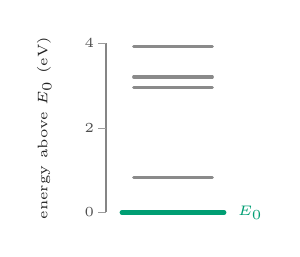
\begin{tikzpicture}\draw[oiInk!55,line width=0.5pt] (0.15,0.15)--(0.15,2.30);\draw[oiInk!45,line width=0.4pt] (0.05,0.15)--(0.15,0.15) node[anchor=east,font=\tiny,text=oiInk!80,xshift=-0.3mm]{0};\draw[oiInk!45,line width=0.4pt] (0.05,1.22)--(0.15,1.22) node[anchor=east,font=\tiny,text=oiInk!80,xshift=-0.3mm]{2};\draw[oiInk!45,line width=0.4pt] (0.05,2.30)--(0.15,2.30) node[anchor=east,font=\tiny,text=oiInk!80,xshift=-0.3mm]{4};\node[rotate=90,anchor=south,font=\tiny,text=oiInk] at (-0.42,1.22) {energy above $E_0$ (eV)};\draw[oiGreen,line width=1.6pt,line cap=round] (0.35,0.15)--(1.65,0.15);\node[anchor=west,font=\tiny,text=oiGreen] at (1.7,0.15) {$E_0$};\draw[oiGrey,line width=1.1pt,line cap=round] (0.5,0.59)--(1.5,0.59);\draw[oiGrey,line width=1.1pt,line cap=round] (0.5,1.74)--(1.5,1.74);\draw[oiGrey,line width=1.1pt,line cap=round] (0.5,1.87)--(1.5,1.87);\draw[oiGrey,line width=1.1pt,line cap=round] (0.5,2.26)--(1.5,2.26);\end{tikzpicture}};
\draw[-{Stealth[length=2.4mm]},oiInk!65,line width=1pt] (12.75,0.9)--(10.60,0.9);
\draw[-{Stealth[length=2.4mm]},oiInk!65,line width=1pt] (6.60,0.9)--(4.65,0.9);
\draw[-{Stealth[length=2.6mm]},oiVerm,line width=1.1pt] (14.65,4.7)--(14.65,3.5);
\node[anchor=west,font=\tiny,text=oiVerm,align=left] at (14.80,4.1) {recovered\\bitstrings};
\draw[oiInk!25,line width=0.5pt] (0,-2.0)--(17.4,-2.0);
\node[anchor=north,font=\footnotesize\bfseries,text=oiInk] at (8.70,-2.15) {Machine-learning entry points};
\node[circle,fill=oiOrange,text=white,font=\tiny\bfseries,inner sep=1.6pt] at (2.2,-2.95) {1};
\node[anchor=west,font=\scriptsize,text=oiInk] at (2.5,-2.95) {design the sampling circuit \emph{(GQE, stage 2)}};
\node[circle,fill=oiPurple,text=white,font=\tiny\bfseries,inner sep=1.6pt] at (9.6,-2.95) {2};
\node[anchor=west,font=\scriptsize,text=oiInk] at (9.9,-2.95) {generate / select configurations --- RBM $\cdot$ NQS $\cdot$ GFlowNet \emph{(stages 4--5)}};
\end{tikzpicture}
}
\caption{\textbf{The sample-based quantum diagonalization workflow, with real data at every stage} (N$_2$, CAS(10e,12o), exact-FCI-verifiable). A shallow LUCJ circuit on the quantum processor (orbital rotations $U(\theta)$ interleaved with diagonal-Coulomb Jastrow gates) is sampled in the computational basis; here $77\%$ of shots survive particle-number post-selection at Heron-calibrated noise. The classical co-processor repairs the broken samples by occupation-weighted S-CORE, assembles the recovered determinants into a subspace $\mathcal{S}$ (each row of panel~5 is one selected configuration's orbital occupation), and diagonalizes the projected Hamiltonian, whose energy is a variational upper bound converging to the exact FCI value (panel~6). Machine learning augments either the sampler (\ent{1}, generative circuit design) or the generation/selection of configurations (\ent{2}). Every panel is real output of the accompanying calculations.}
\label{fig:loop}
\end{figure*}

The object shared by all methods in this review is a hybrid quantum--classical loop with four stages. (i) A parameterized quantum circuit prepares an approximate ground state. In the flagship demonstrations this is the \emph{local unitary cluster Jastrow} (LUCJ) ansatz \cite{motta2023}, a hardware-efficient truncation of unitary coupled cluster that alternates orbital rotations with diagonal Coulomb (Jastrow) factors and restricts entangling operations to a physically motivated local connectivity, making it native to heavy-hex superconducting lattices and initializable from classical CCSD amplitudes. (ii) The circuit is measured in the computational basis; under the Jordan--Wigner mapping each length-$2M$ bitstring (for $M$ spatial orbitals) is an electronic configuration, split into an $\alpha$ and a $\beta$ half. Each measured bitstring is thus a \emph{proposed} Slater determinant, and the collection of distinct bitstrings, with their frequencies, is the raw material the rest of the pipeline processes. (iii) In SQD, noise corrupts a large fraction of these bitstrings to the wrong particle number or spin; a \emph{self-consistent configuration recovery} (S-CORE) step repairs them, flipping spin-orbitals toward the mean occupation of the current best eigenvector and iterating to self-consistency \cite{robledomoreno2025}; we make the mechanism precise below. (iv) The Hamiltonian is projected onto the recovered determinant subspace and diagonalized by a sparse (Davidson) eigensolver, distributed across high-performance classical hardware; the result is a variational upper bound and a sparse ground-state wavefunction.

Formally, the electronic Hamiltonian in second quantization is

\begin{equation}
\hat H \;=\; \sum_{pq} h_{pq}\, \hat a_p^{\dagger}\hat a_q \;+\; \tfrac{1}{2}\!\sum_{pqrs} (pq|rs)\, \hat a_p^{\dagger}\hat a_r^{\dagger}\hat a_s\hat a_q \;+\; E_{\mathrm{nuc}},
\end{equation}

whose exact diagonalization in the full configuration-interaction (FCI) basis of $M$ active spatial orbitals with $(n_\alpha,n_\beta)$ electrons has dimension $\dim\mathcal H_{\mathrm{FCI}} = \binom{M}{n_\alpha}\binom{M}{n_\beta}$, growing combinatorially. SQD replaces $\mathcal H_{\mathrm{FCI}}$ by a sampled subspace $\mathcal S = \mathrm{span}\{|D_x\rangle\}_{x\in\mathcal S}$ of Slater determinants and solves the projected eigenproblem for the projector $\hat P_{\mathcal S}=\sum_{x\in\mathcal S}|D_x\rangle\langle D_x|$,

\begin{equation}
\big(\hat P_{\mathcal S}\,\hat H\,\hat P_{\mathcal S}\big)\,\mathbf c \;=\; E_{\mathcal S}\,\mathbf c, \qquad E_{\mathcal S} \;\ge\; E_{\mathrm{FCI}},
\end{equation}

the inequality (the Hylleraas--Undheim--MacDonald theorem) being the variational guarantee that makes every SQD energy a rigorous upper bound that improves monotonically as good determinants are added. This guarantee is a double-edged asset, and the edge it cuts against is the theme of \S\ref{sec:5}--\S\ref{sec:7}: the same projected-Hamiltonian structure that lets one \emph{certify} an SQD energy from the classical side is what lets one \emph{construct}, screen, and, for the shallow circuits actually run, \emph{simulate} the subspace classically. The variational principle that grounds the method's appeal is thus also the doorway through which its classical competitors enter. The self-consistent recovery (S-CORE) closes the loop: from the current subspace eigenvector it forms the mean spin-orbital occupations $\langle n_p\rangle = \sum_{x\in\mathcal S} |c_x|^2\, [x]_p$ and repairs each symmetry-broken bitstring by flipping spin-orbitals with probability increasing in the deviation $\big|[x]_p-\langle n_p\rangle\big|$, iterating recovery $\to$ diagonalization $\to$ occupation-update to self-consistency. Because the whole quantitative analysis of this review lives in an active space small enough for exact FCI (N$_2$ and H$_2$O in CAS(10e,12o)/(8e,12o), whose active-space orbitals are shown in Fig.~\ref{fig:system}), every energy we quote below is an \emph{error against exact truth} within that model space, not against another approximation.


\begin{figure*}[tb]
\centering

\includegraphics[width=1.0\linewidth]{pf_system.pdf}
\caption{\textbf{The molecular systems, their active-space orbital-energy structure, and the frontier orbitals.} \emph{(a,f)} Ray-traced ball-and-stick geometries of stretched N$_2$ ($R=2.0\,$Å, CAS(10e,12o)) and H$_2$O (CAS(8e,12o)). \emph{(b,g)} Molecular-orbital energy-level diagrams (restricted Hartree--Fock, eV): occupied active levels (blue) carry their two electrons as up/down arrows, virtual active levels are red, the shaded band is the complete active space, and $E_F$ marks the HOMO--LUMO midpoint; the deep $1s$ core is frozen and off-scale. \emph{(c--e)} Ray-traced (PyMOL) isosurfaces of the N$_2$ frontier orbitals --- the two-fold-degenerate $1\pi_u$ HOMO ($-10.9$~eV; note the axis-containing nodal plane of $\pi$ symmetry), the non-degenerate $3\sigma_g$ level just below it ($-13.0$~eV; cylindrically symmetric about the bond axis), and the $1\pi_g^{*}$ LUMO ($-2.3$~eV) --- with their RHF energies. The crowding of these frontier levels as the triple bond stretches, and the collapse of the bonding--antibonding gaps ($1\pi_u/1\pi_g^{*}$, $3\sigma_g/3\sigma_u^{*}$) toward dissociation, is what makes stretched N$_2$ strongly multireference: at $R=2.0$~\AA{} the FCI natural-orbital occupations of the frontier pair are already $1.32/0.68$ (versus the closed-shell $2/0$) and the Hartree--Fock determinant carries only $34\%$ of the exact weight (\S\ref{sec:7}). \emph{(h,i)} The H$_2$O $1b_1$ lone-pair HOMO and $4a_1^{*}$ LUMO. Isosurfaces at $|\psi|=0.028\,a_0^{-3/2}$; orbital phases orange/blue.}
\label{fig:system}
\end{figure*}

Two lineages coined the idea nearly simultaneously and use different names for it. \emph{Quantum-selected configuration interaction} (QSCI) was introduced by Kanno and co-workers \cite{kanno2023}, now published in \emph{Physical Review Research}, and framed the method as ``the quantum computer selects the subspace, the classical computer diagonalizes.'' \emph{Sample-based quantum diagonalization} (SQD) is the IBM--RIKEN realization at quantum-centric-supercomputing scale \cite{robledomoreno2025}, adding the self-consistent recovery loop and the tight coupling to an HPC back end. We use SQD and QSCI interchangeably, noting the recovery step as the principal methodological difference and the natural home of the machine-learning contributions reviewed in \S\ref{sec:4}. Crucially, because the final step is an exact diagonalization in a fixed subspace, the energy is variational: it can only be an upper bound to the true ground state, and it improves monotonically as good determinants are added --- a property that both grounds the method's appeal and, as \S\ref{sec:5} will show, sets the exact bar its classical competitors must be measured against.


\subsection{A taxonomy of variants}\label{sec:2-2}

In two years the SQD/QSCI family has branched into some fifty distinct variants; we organize them by the stage of the loop they modify (Table~\ref{tab:sqd}). \emph{Input-state variants} replace the LUCJ sampler: ADAPT-QSCI grows the state one Pauli generator at a time without a variational optimization \cite{nakagawa2024}; time-evolved QSCI (TE-QSCI) and Hamiltonian-simulation QSCI (HSB-QSCI) generate multi-order excitations from real-time evolution rather than circuit optimization \cite{mikkelsen2025,sugisaki2025}; and generative circuit design learns the sampler itself (\S\ref{sec:4-5}). \emph{Krylov variants} (sample-based Krylov quantum diagonalization, SKQD, and its randomized provable-convergence descendant SqDRIFT) build a Krylov subspace from sampled time-evolved states, importing phase-estimation-like convergence guarantees at low depth \cite{yu2025,piccinelli2025}. \emph{Recovery and selection variants} attack the coupon-collector bottleneck directly: amplitude amplification of unseen bitstrings \cite{stockinger2026}, active-sampling by an Epstein--Nesbet acquisition function \cite{miura2026}, and (the focus of \S\ref{sec:4}) machine-learned recovery. \emph{Qubit-reduced variants} halve the register through half-qubit encodings, seniority-zero sampling, entanglement forging, or neural fermionic compression \cite{mcfarthing2026,yoshida2026,smith2025,chen2025}, and a CI-matrix reformulation (CIM-QSCI) pushes further to a logarithmic $\lceil\log_2 N\rceil$ qubit count \cite{graves2026}. \emph{Embedding variants} reach extended systems by using SQD as the impurity or fragment solver inside density-matrix embedding, localized-active-space SCF, or DFT embedding \cite{shajan2025,wang2026}. \emph{Hybrid post-processing variants} recover dynamical correlation missed by the finite subspace, using the SQD wavefunction as an AFQMC trial, a tailored-CC reference, or a multireference-PT2 anchor \cite{danilov2025,erhart2025}. A full annotated tabulation, with citations, systems, and largest scale, is given in the accompanying dataset.



\begin{table*}[t]\centering\footnotesize
\caption{The SQD/QSCI method family (curated; the full annotated list is maintained in the state-of-the-art dataset). ``Largest scale'' states hardware qubit counts or active spaces as reported.}
\label{tab:sqd}
\renewcommand{\arraystretch}{1.25}
\begin{tabularx}{\textwidth}{@{}>{\raggedright\arraybackslash}p{2.6cm} >{\raggedright\arraybackslash}p{2.0cm} >{\raggedright\arraybackslash}X >{\raggedright\arraybackslash}p{2.4cm} >{\raggedright\arraybackslash}p{1.8cm}@{}}
\toprule
\textbf{Category} & \textbf{Method} & \textbf{Key idea} & \textbf{Ref.} & \textbf{Largest scale} \\
\midrule
Core & QSCI & Quantum samples the subspace; classical diagonalization & \cite{kanno2023} & 8 qubits \\
 & SQD + S-CORE & Self-consistent configuration recovery; quantum-centric supercomputing & \cite{robledomoreno2025} & 77\,q / (54e,36o) \\
Sampler/input & ADAPT-QSCI & Iterative input-state growth, no VQE & \cite{nakagawa2024} & small molecules \\
 & TE-/HSB-QSCI & Time-evolved / Hamiltonian-simulation sampling state & \cite{mikkelsen2025,sugisaki2025} & 36\,q (carbyne) \\
 & Generative-QSCI & Transformer (GQE) designs the sampling circuit & \cite{kemmoku2026} & 32\,q (N$_2$) \\
Krylov & SKQD / SqDRIFT & Sampled Krylov subspace; provable convergence & \cite{yu2025,piccinelli2025} & 49\,q \\
Recovery/select & SQD-AA & Amplitude-amplify unseen bitstrings (quadratic gain) & \cite{stockinger2026} & model systems \\
 & ML recovery & Learned generation/classification (see Table~\ref{tab:ml}) & --- & see Table~\ref{tab:ml} \\
Excited/orbital & ext-/oo-SQD & Extra projection for excited states; orbital optimization & \cite{barison2025} & CH$_2$ 52\,q \\
Symmetry/compact & Compact-QSCI & Space-group symmetry; time-evolved compact subspaces & \cite{weaving2025,nogaki2026} & SiH$_4$ 42\,q \\
Qubit-reduced & HCI-HSQD & Half-qubit; seniority-zero; neural compression & \cite{mcfarthing2026} & Fe-S (54e,36o) \\
Embedding & DMET-/LAS-SQD & SQD as fragment / impurity solver & \cite{wang2026} & protein 12{,}635 atoms \\
Hybrid post-proc. & AFQMC-SQD; PT2 & Recover dynamical correlation on the SQD reference & \cite{danilov2025,erhart2025} & N$_2$; [2Fe-2S] \\
\bottomrule
\end{tabularx}
\end{table*}

\subsection{Hardware demonstrations and honest scale}\label{sec:2-3}

The method's hardware trajectory is genuinely impressive and worth stating precisely, because it is often conflated with an advantage claim it does not make. The founding demonstration reached N$_2$ at 58 qubits and the iron--sulfur clusters [2Fe-2S] and [4Fe-4S] on 45- and 77-qubit registers, with classical diagonalization distributed across up to 6,400 nodes of Fugaku \cite{robledomoreno2025}; the [4Fe-4S] run, a (54e,36o) active space (72 Jordan--Wigner spin-orbitals, the balance of the register serving the heavy-hex LUCJ mapping), was the largest quantum-computed at the time. A full-scale closed-loop follow-up used the entire 152,064-node Fugaku machine with an on-premises Heron processor and improved the [4Fe-4S] energy by 278 mHa over the 2024 result \cite{shirakawa2025}. Fragment-based embeddings then pushed the workflow, in 2025--2026, from a $\sim$300-atom miniprotein to a 12,635-atom protein--ligand complex \cite{wang2026}. These are landmark demonstrations of \emph{scale beyond exact diagonalization}. They are not, and are not claimed by their authors to be, demonstrations of an advantage over the best classical methods, a distinction \S\ref{sec:5} makes central.


\subsection{Software and ecosystem}\label{sec:2-4}

The method is unusually well tooled for its age, which partly explains its rapid uptake. IBM maintains \texttt{qiskit-addon-sqd} (with an HPC C++ variant) and \texttt{ffsim} for fermionic-circuit simulation and LUCJ construction; QunaSys maintains \texttt{quri-parts-qsci} within the QURI SDK and, notably, a continuously updated community bibliography, \emph{Awesome-QSCI}, that functions as a living review of a field moving too fast for the conventional publication cycle. NVIDIA's CUDA-Q documents SKQD as a reference application and provides GPU primitives for the classical diagonalization back end. This tooling maturity is a mixed blessing: it lowers the barrier to method development --- including the machine-learning methods of \S\ref{sec:4} --- but it also lowers the barrier to producing demonstrations that are not benchmarked against the strong classical baselines of \S\ref{sec:5}.


\section{The configuration-recovery bottleneck: the machine-learning entry point}\label{sec:3}


\subsection{A coupon-collector law}\label{sec:3-1}

The efficiency of the entire loop reduces to a single question: how many distinct, \emph{important} determinants can be placed in the subspace, and at what cost? The answer is governed by the amplitude distribution of the exact ground state, which is heavy-tailed. In stretched N$_2$ in a (10e,12o) active space, for instance, 90\% of the exact FCI weight is carried by roughly 1.4\% of the single-spin strings (about a dozen of the 792), with per-configuration weights spanning many orders of magnitude. Sampling from such a distribution to \emph{discover} the low-amplitude but chemically decisive determinants is a coupon-collector problem with non-uniform probabilities: as sampling proceeds, an overwhelming fraction of draws re-select already-seen configurations, and the number of newly discovered determinants per shot collapses. Reinholdt and co-workers made this quantitative and damaging: for N$_2$ the discovery rate falls from $\sim$0.1 determinants per shot at $10^3$ shots to $\sim\!5\times10^{-4}$ at $10^9$, and reaching micro-hartree precision extrapolates to on the order of $10^{14}$ samples \cite{reinholdt2025}. This is the bottleneck that machine learning is invoked to break: if a learned model can \emph{generate} the important tail rather than wait to sample it, the coupon-collector wall might be circumvented. Whether it can --- and whether doing so beats simply running a classical selected-CI heuristic --- is the question of \S\ref{sec:4} and \S\ref{sec:5}.

The effect is exact and computable. Writing the marginal weight of a single-spin string $i$ as $w_\alpha(i)=\sum_\beta|c_{i\beta}|^2$ and its sampling probability as $p_i$, the expected number of shots required to first observe every string in a target set $\mathcal T$ is bounded above by the coupon-collector sum (the leading inclusion--exclusion term, tight in the heavy-tail regime the argument invokes)

\begin{equation}
\mathbb E\big[\,\text{shots to collect } \mathcal T\,\big] \;\le\; \sum_{i\in\mathcal T}\frac{1}{p_i} \;\xrightarrow[\;p_i\to 0\;]{}\; \infty,
\end{equation}

which upper-bounds the exact expectation (the leading term of an inclusion--exclusion series) and diverges as the heavy tail is approached. Fig.~\ref{fig:coupon} computes this directly from the exact FCI wavefunction of N$_2$ CAS(10e,12o): the same handful of dominant strings carry almost all the weight, but the correlation-energy tail that decides chemical accuracy is spread over hundreds of rare strings --- precisely the configurations whose $p_i$ make the sum above large, and precisely where a learned generator is supposed to earn its keep.


\begin{figure*}[tb]
\centering
\begin{tikzpicture}
\begin{groupplot}[group style={group size=2 by 1, horizontal sep=2.4cm}, paperplot, width=0.46\linewidth, height=0.40\linewidth]
% ================= Panel a : heavy-tailed weights =================
\nextgroupplot[ymode=log, xlabel={single-spin string, ranked by weight}, ylabel={marginal weight $w_\alpha(i)$},
  xmin=0, xmax=792, ymin=1e-9, ymax=0.6, ytick={1e0,1e-2,1e-4,1e-6,1e-8}, ymajorgrids, clip=false,
  title={heavy-tailed determinant weights (N$_2$, exact FCI)}]
  \addplot[draw=none, fill=oiOrange!13, forget plot] table[x=rank,y=weight]{coupon_w.dat} \closedcycle;
  \addplot[oiBlue, line width=1pt] table[x=rank,y=weight]{coupon_w.dat};
  \draw[oiOrange, densely dashed, line width=1pt] (axis cs:11,1e-9) -- (axis cs:11,0.55);
  \node[oiOrange!80!black, font=\scriptsize, anchor=west, align=left] at (axis cs:95,6e-2){90\% weight in\\11 strings};
  \draw[-{Stealth[length=1.7mm]}, oiOrange!80!black, line width=0.7pt] (axis cs:90,7e-2) -- (axis cs:15,1.3e-2);
  \node[oiOrange!65!black, font=\scriptsize, anchor=west] at (axis cs:140,2.4e-8){correlation-energy tail};
  \node[font=\bfseries\large, anchor=south east] at (rel axis cs:-0.14,1.0){a};
% ================= Panel b : coupon-collector signature =================
\nextgroupplot[xlabel={number of strings included}, ylabel={cumulative ground-state weight},
  xmin=0, xmax=260, ymin=0, ymax=1.04, ytick={0,0.2,0.4,0.6,0.8,1.0}, title={the coupon-collector signature}, clip=false]
  \addplot[oiGreen, line width=1.4pt] table[x=n,y=cum]{coupon_cum.dat};
  \addplot[only marks, mark=*, mark size=3pt, color=oiOrange, forget plot] coordinates {(11,0.9025)};
  \addplot[only marks, mark=*, mark size=3pt, color=oiVerm, forget plot] coordinates {(47,0.9901)};
  \addplot[only marks, mark=*, mark size=3pt, color=oiPurple, forget plot] coordinates {(187,0.9990)};
  \node[oiOrange!88!black, font=\scriptsize\bfseries, anchor=west] at (axis cs:20,0.46){90.2\% of weight $\rightarrow$ 11 strings (1.4\%)};
  \node[oiVerm, font=\scriptsize\bfseries, anchor=west] at (axis cs:20,0.33){99.0\% $\rightarrow$ 47 strings (5.9\%)};
  \node[oiPurple, font=\scriptsize\bfseries, anchor=west] at (axis cs:20,0.20){99.9\% $\rightarrow$ 187 strings (23.6\%)};
  \node[font=\bfseries\large, anchor=south east] at (rel axis cs:-0.14,1.0){b};
\end{groupplot}
\end{tikzpicture}
\caption{\textbf{The coupon-collector bottleneck, computed exactly.} N$_2$ CAS(10e,12o), from the exact FCI wavefunction. \emph{Left:} the marginal single-spin-string weight $w_\alpha(i)=\sum_\beta|c_{i\beta}|^2$ falls across roughly eight orders of magnitude, from $0.35$ down to ${\sim}10^{-9}$. \emph{Right:} $90\%$ of the ground-state weight is carried by about a dozen of the $792$ strings (roughly $1.4\%$), but the correlation-energy tail is spread over hundreds of rare strings --- the configurations a sampler must pay to discover.}
\label{fig:coupon}
\end{figure*}


\subsection{Recovery as denoising, and the peculiar role of noise}\label{sec:3-2}

On real hardware the bottleneck is compounded by noise, and here the picture is subtle in a way that is central to the field's clear-eyed self-assessment. Under readout and gate noise, the majority of measured bitstrings violate particle-number conservation and would be discarded by naive post-selection: for N$_2$ in a large active space on hardware, only about 0.17\% of raw samples survive \cite{vaquerosabater2026}. This survival fraction falls steeply with register width, since each additional qubit is another channel for a particle-number-violating readout error: our illustrative $12$-orbital N$_2$ CAS retains ${\sim}77\%$ of shots at $1\times$ Heron noise (Fig.~\ref{fig:loop}), whereas a large hardware active space over many more qubits retains a fraction of a percent, the same mechanism two orders of magnitude apart in scale. The self-consistent configuration recovery step is precisely a statistical imputation model that rescues these corrupted samples, and it is the true workhorse of SQD's noise tolerance. Strikingly, Vaquero-Sabater and co-workers showed that noise can \emph{help}: by scattering samples beyond the biased support of the ideal ansatz, moderate noise broadens Hilbert-space exploration, and recovery starting from \emph{uniformly random} bitstrings reaches accurate energies within a couple of iterations. The implication, that the classical recovery loop (not the quantum sampler) is responsible for the accuracy, is one of the sharpest results in the literature and is examined in \S\ref{sec:5}. For the present section the point is narrower: the recovery step is a learned/statistical model, and it is the natural site for the generative methods of \S\ref{sec:4}, whose promise is to replace an occupancy-weighted heuristic repair with a model that has learned the structure of the important subspace. Fig.~\ref{fig:score} makes the mechanism concrete on backend-calibrated noise: as the device-noise scale grows the fraction of particle-number-valid shots collapses, yet S-CORE recovery still lowers the fixed-dimension subspace error by imputing the broken samples back onto valid configurations, with its largest benefit at moderate noise.


\begin{figure*}[tb]
\centering
\begin{tikzpicture}
\begin{groupplot}[group style={group size=2 by 1, horizontal sep=2.1cm}, paperplot, width=0.46\linewidth, height=0.40\linewidth]
\nextgroupplot[xlabel={noise scale ($\times$ FakeTorino/Heron)}, ylabel={valid shots lost (\%)},
  xmin=-0.12, xmax=3.12, ymin=0, ymax=60, xtick={0,1,2,3}, title={noise destroys particle-number conservation},
  nodes near coords={\pgfmathprintnumber[precision=0]{\pgfplotspointmeta}\%},
  nodes near coords style={font=\scriptsize, text=oiVerm!75!black, anchor=south east, xshift=-1pt}, clip=false]
  \addplot[draw=none, fill=oiVerm!10, forget plot] table[x=scale,y=lost]{recovery.dat} \closedcycle;
  \addplot[oiVerm, line width=1.4pt, mark=*, mark size=3pt, mark options={fill=oiVerm,draw=white}] table[x=scale,y=lost]{recovery.dat};
  \node[font=\bfseries\large, anchor=south east] at (rel axis cs:-0.16,1.0){a};
\nextgroupplot[xlabel={noise scale}, ylabel={subspace energy error (mHa)},
  xmin=-0.12, xmax=3.12, ymin=26, ymax=35, xtick={0,1,2,3}, ytick={26,28,30,32,34}, title={S-CORE rescues the subspace ($D=120$)},
  legend style={at={(0.5,-0.30)}, anchor=north, legend columns=1}, clip=false]
  \addplot[name path=raw, oiGrey, line width=1.3pt, mark=square*, mark size=2.6pt, mark options={fill=oiGrey,draw=white},
    nodes near coords, nodes near coords style={font=\scriptsize, text=oiInk!65, anchor=south, yshift=1.5pt, /pgf/number format/fixed, /pgf/number format/precision=1}]
    table[x=scale,y=eraw]{recovery.dat}; \addlegendentry{raw (discard invalid shots)}
  \addplot[name path=rec, oiGreen, line width=1.3pt, mark=*, mark size=2.6pt, mark options={fill=oiGreen,draw=white},
    nodes near coords, nodes near coords style={font=\scriptsize, text=oiGreen!55!black, anchor=north, yshift=-1.5pt, /pgf/number format/fixed, /pgf/number format/precision=1}]
    table[x=scale,y=erec]{recovery.dat}; \addlegendentry{after S-CORE recovery}
  \addplot[oiGreen!18, forget plot] fill between[of=raw and rec];
  \node[font=\bfseries\large, anchor=south east] at (rel axis cs:-0.17,1.0){b};
\end{groupplot}
\end{tikzpicture}
\caption{\textbf{Configuration recovery under backend-calibrated noise} (FakeTorino / Heron r1 rates; asymmetric readout $+$ depolarizing). \emph{Left:} the fraction of particle-number-valid shots collapses as the noise scale grows. \emph{Right:} at fixed dimension $D=120$, S-CORE recovery (green) lowers the subspace energy error relative to discarding the invalid shots (grey) --- most at moderate noise ($\sim$3~mHa at $1\times$, shrinking to $\sim$0.3~mHa at $3\times$) --- while the raw curve (grey) drifts steadily downward and the recovered curve (green) drops sharply then stays low as noise broadens Hilbert-space exploration, both consistent with the ``noise can help'' effect. Note the recovered subspace stays well above chemical accuracy here ($\sim$28--34~mHa at this fixed, illustrative $D$): recovery salvages otherwise-discarded samples, it does not by itself reach chemical precision.}
\label{fig:score}
\end{figure*}


\subsection{Why the standard error-mitigation toolkit does not transfer}\label{sec:3-3}

A methodological subtlety that the field has had to internalize, and that a review should make explicit, is that SQD is a \emph{per-sample} post-selection pipeline, not an expectation-value pipeline. This distinction determines which of the near-term error-mitigation techniques transfer. Post-selection on particle number and spin, self-consistent recovery, and symmetry projection via classical shadows \cite{huang2020} operate on individual bitstrings and are central to the method. In contrast, the techniques that dominate IBM's utility-scale expectation-value experiments (twirled readout error extinction, TREX; zero-noise extrapolation, ZNE; and probabilistic error cancellation, PEC) mitigate errors \emph{in expectation values}, not in individual samples, and therefore do not transfer to a pipeline that needs valid configurations rather than corrected averages. Dynamical decoupling and Pauli twirling give only marginal, inconsistent benefit once the recovery loop has converged \cite{bhuiyan2026}. The practical consequence, relevant to \S\ref{sec:6}, is that a claim about SQD's hardware performance must be benchmarked with the mitigation stack it actually uses (recovery + symmetry post-selection), not the expectation-value stack, and that the shot budget saturates surprisingly early, optimal at $10^3$--$10^4$ shots, with $10^5$ performing \emph{worse} \cite{bhuiyan2026}. This early hardware saturation does not contradict the ${\sim}10^{14}$-sample extrapolation of \S\ref{sec:3-1}: that figure is the noiseless discovery limit for the exact heavy tail, whereas this one is the point at which, on noisy hardware with recovery already converged, additional shots mostly re-collect configurations the recovery step has restored rather than discovering new tail determinants.


\section{Machine learning and generative methods for determinant and subspace selection}\label{sec:4}

The proposition uniting this section is simple to state: if the important determinants are heavy-tailed and expensive to discover by sampling (\S\ref{sec:3-1}), replace or augment the raw sampler with a \emph{model} that has learned where they are. The proposition is also older than SQD: Coe's machine-learning configuration interaction (MLCI) trained a neural network on-the-fly to predict which unseen determinants a classical selected-CI loop should add, on CO and stretched water, as early as 2018 \cite{coe2018,coe2019}. What SQD added is a reason to revisit the idea urgently and at scale, and a quantum sampler to compete with or complement. The result is a fast-moving ecosystem that, to our knowledge, has not been surveyed. We organize it along two axes, the \emph{object} a method generates (a determinant, a subspace, a circuit) and the \emph{importance signal} it is trained on (CI-coefficient magnitude, a perturbative estimate, quantum-sample frequency, or the diagonalized energy itself), and we treat the four families in turn, closing with the conspicuous gap the taxonomy exposes.


\subsection{A taxonomy by generated object and importance signal}\label{sec:4-1}


\begin{figure*}[tb]
\centering
\resizebox{\linewidth}{!}{%
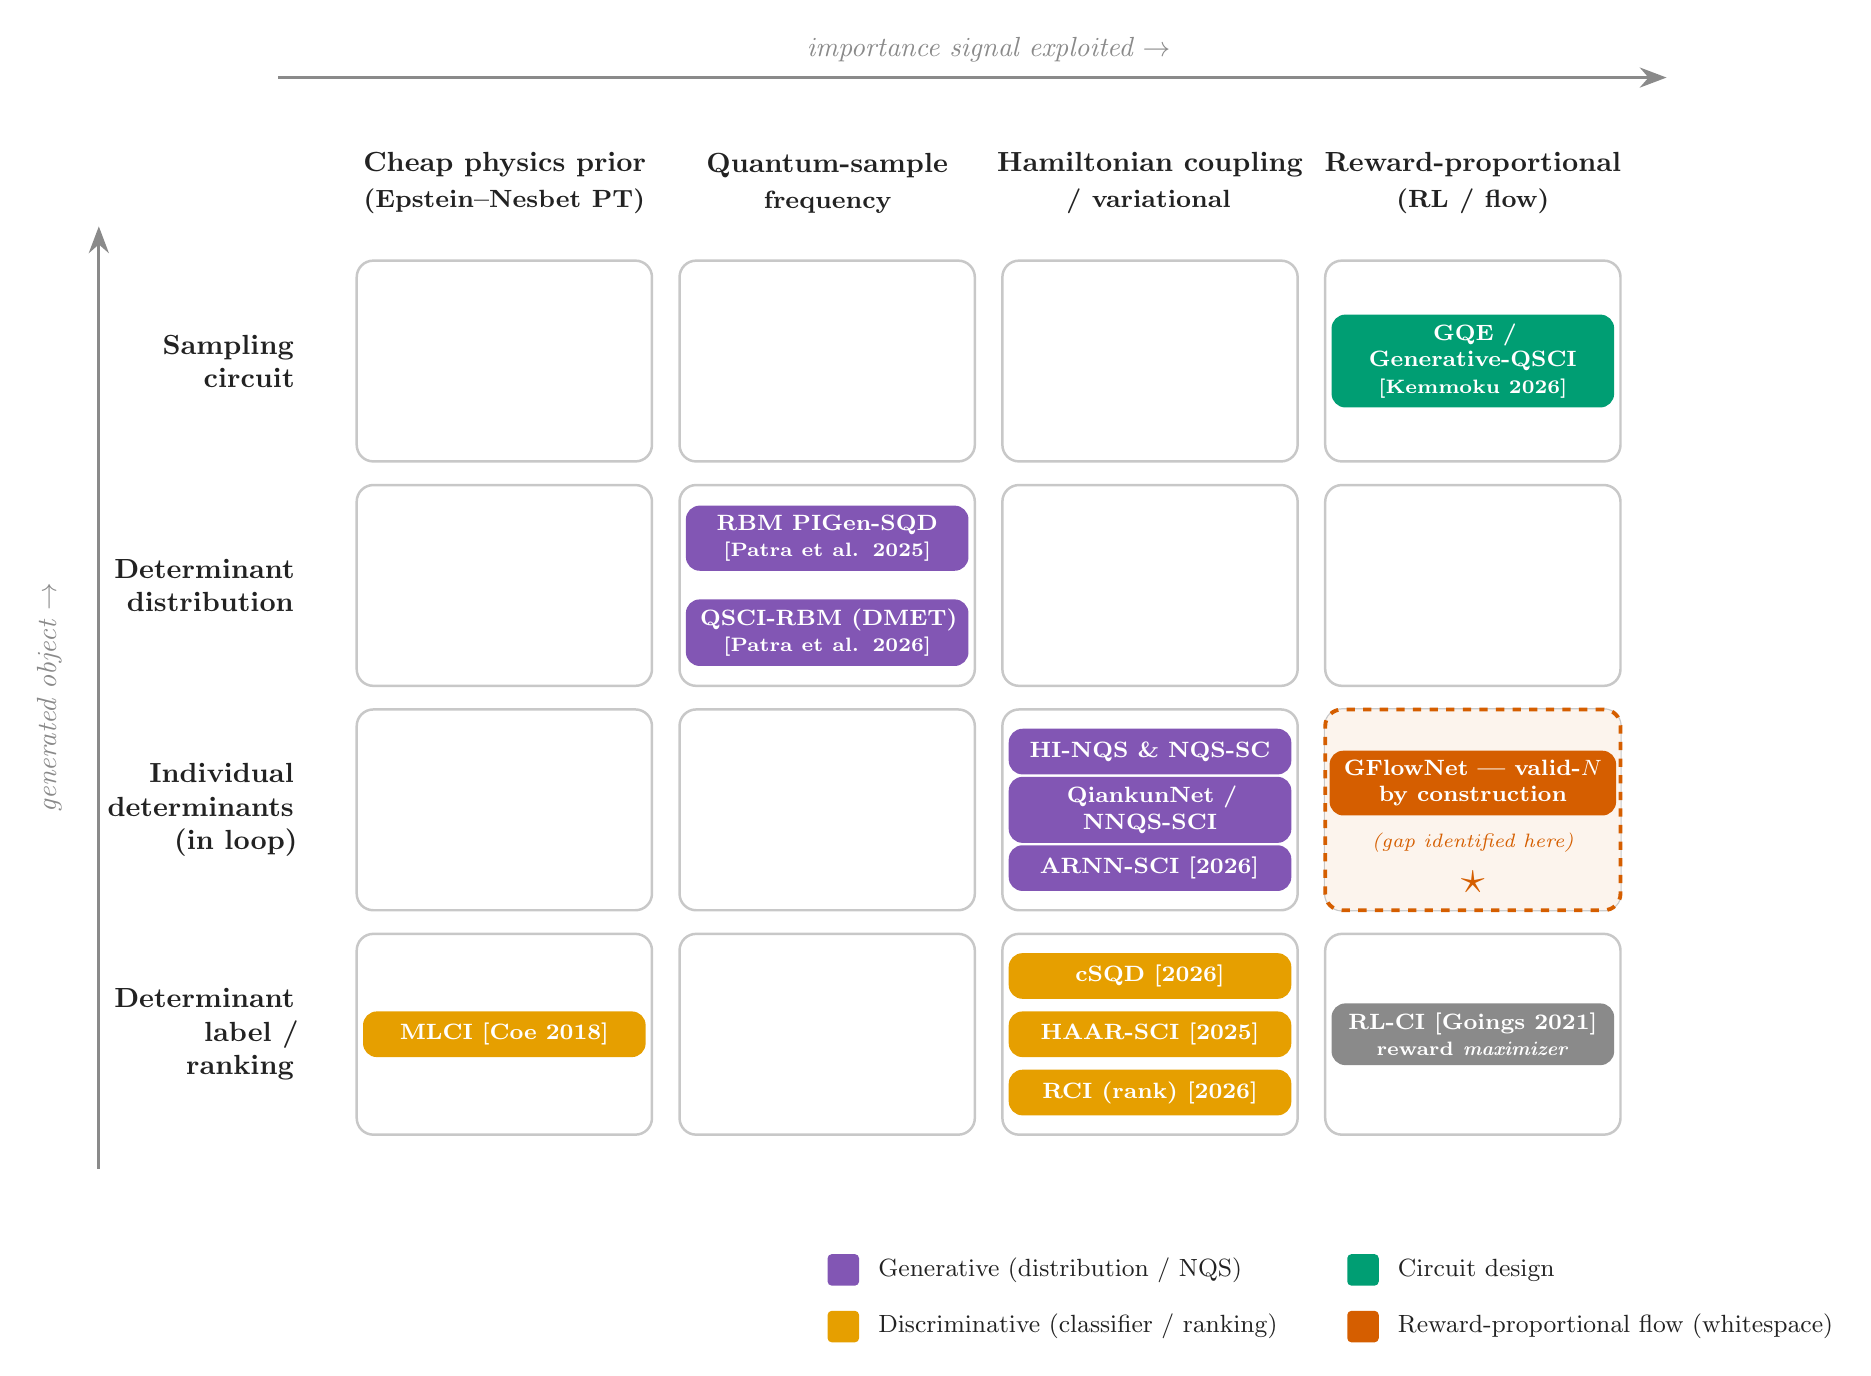
\begin{tikzpicture}[font=\sffamily,
  cell/.style={draw=oiInk!25, rounded corners=6pt, line width=0.9pt, minimum width=3.75cm, minimum height=2.55cm},
  wscell/.style={draw=oiVerm, dashed, line width=1.4pt, fill=oiVerm!7, rounded corners=6pt, minimum width=3.75cm, minimum height=2.55cm},
  chip/.style={rounded corners=5pt, text=white, font=\footnotesize\bfseries, align=center, inner sep=3.4pt, minimum height=0.58cm, text width=3.35cm},
  chipT/.style={rounded corners=5pt, text=white, font=\footnotesize\bfseries, align=center, inner sep=3.4pt, minimum height=0.78cm, text width=3.35cm},
  colh/.style={font=\bfseries, text=oiInk, align=center, text width=4.0cm, anchor=south},
  rowh/.style={font=\bfseries, text=oiInk, align=right, text width=2.5cm, anchor=east},
]
\def\cx{4.1}\def\cy{2.85}
% ---- grid ----
\foreach \c in {0,1,2,3}{\foreach \r in {0,1,2,3}{\node[cell] at (\c*\cx,\r*\cy){};}}
\node[wscell] at (3*\cx,1*\cy){};
% ---- column headers (anchored above the grid) ----
\def\hy{10.30}
\node[colh] at (0*\cx,\hy){Cheap physics prior\\[1pt]{\small (Epstein--Nesbet PT)}};
\node[colh] at (1*\cx,\hy){Quantum-sample\\[1pt]{\small frequency}};
\node[colh] at (2*\cx,\hy){Hamiltonian coupling\\[1pt]{\small / variational}};
\node[colh] at (3*\cx,\hy){Reward-proportional\\[1pt]{\small (RL / flow)}};
% ---- row headers ----
\node[rowh] at (-2.55,3*\cy){Sampling\\circuit};
\node[rowh] at (-2.55,2*\cy){Determinant\\distribution};
\node[rowh] at (-2.55,1*\cy){Individual\\determinants\\(in loop)};
\node[rowh] at (-2.55,0*\cy){Determinant\\label / ranking};
% ---- chips ----
\node[chipT,fill=oiGreen] at (3*\cx,3*\cy){GQE / Generative-QSCI\\{\scriptsize [Kemmoku 2026]}};
\node[chipT,fill=oiPurple] at (1*\cx,2*\cy+0.60){RBM PIGen-SQD\\{\scriptsize [Patra et al. 2025]}};
\node[chipT,fill=oiPurple] at (1*\cx,2*\cy-0.60){QSCI-RBM (DMET)\\{\scriptsize [Patra et al. 2026]}};
\node[chip,fill=oiPurple] at (2*\cx,1*\cy+0.74){HI-NQS \& NQS-SC};
\node[chip,fill=oiPurple] at (2*\cx,1*\cy){QiankunNet / NNQS-SCI};
\node[chip,fill=oiPurple] at (2*\cx,1*\cy-0.74){ARNN-SCI [2026]};
\node[chip,fill=oiOrange] at (0*\cx,0*\cy){MLCI [Coe 2018]};
\node[chip,fill=oiOrange] at (2*\cx,0*\cy+0.74){cSQD [2026]};
\node[chip,fill=oiOrange] at (2*\cx,0*\cy){HAAR-SCI [2025]};
\node[chip,fill=oiOrange] at (2*\cx,0*\cy-0.74){RCI (rank) [2026]};
% reward column, maximizer half (RL-CI) --- contrasts the reward-proportional whitespace above it
\node[chipT,fill=oiGrey] at (3*\cx,0*\cy){RL-CI [Goings 2021]\\{\scriptsize reward \emph{maximizer}}};
% whitespace occupant: GFlowNet chip + star below
\node[chipT,fill=oiVerm,text width=3.4cm] at (3*\cx,1*\cy+0.34){GFlowNet --- valid-$N$\\by construction};
\node[oiVerm,font=\itshape\scriptsize] at (3*\cx,1*\cy-0.42){(gap identified here)};
\node[text=oiVerm] at (3*\cx,1*\cy-0.92){\fontsize{18}{18}\selectfont$\star$};
% ---- axis guides ----
\draw[-{Stealth[length=3.4mm]}, oiGrey, line width=1.1pt] (-0.7*\cx,12.15) -- (3.6*\cx,12.15);
\node[oiGrey, font=\itshape, anchor=south] at (1.5*\cx,12.23){importance signal exploited $\rightarrow$};
\draw[-{Stealth[length=3.4mm]}, oiGrey, line width=1.1pt] (-5.15,-0.6*\cy) -- (-5.15,3.6*\cy);
\node[oiGrey, font=\itshape, rotate=90, anchor=south] at (-5.5,1.5*\cy){generated object $\rightarrow$};
% ---- legend ----
\begin{scope}[shift={(1.05*\cx,-1.05*\cy)}]
  \foreach \i/\col/\lab in {0/oiPurple/{Generative (distribution / NQS)}, 1/oiGreen/{Circuit design}, 2/oiOrange/{Discriminative (classifier / ranking)}, 3/oiVerm/{Reward-proportional flow (whitespace)}}{
    \pgfmathsetmacro\lx{mod(\i,2)*6.6}\pgfmathsetmacro\ly{-int(\i/2)*0.72}
    \node[fill=\col, minimum size=4mm, rounded corners=1.5pt] at (\lx,\ly){};
    \node[anchor=west, font=\small, text=oiInk] at (\lx+0.32,\ly){\lab};
  }
\end{scope}
\end{tikzpicture}%
}
\caption{\textbf{A taxonomy of machine-learning methods for determinant and subspace selection in SQD}, organized by the object each method generates (rows) and the importance signal it exploits (columns). Generative models (purple) learn a distribution over determinants; discriminative models (orange) classify or rank them; circuit-design methods (green) learn the sampler itself. The reward-driven column (right) is occupied only by the reinforcement-learning \emph{maximizer} RL-CI [Goings 2021] (grey); the reward-\emph{proportional} flow cell (dashed) that diverse tail discovery calls for is the methodological whitespace this review identifies --- a generative-flow network that constructs valid-$N$ determinants in the loop, unoccupied as of mid-2026.}
\label{fig:taxonomy}
\end{figure*}

Table~\ref{tab:ml} and Fig.~\ref{fig:taxonomy} arrange the methods on the two axes. Two observations organize the rest of the section. First, the field is converging, from several directions, on a single algorithmic skeleton: \emph{propose configurations, diagonalize in their span, use the result to improve the proposer, iterate}. This is not a coincidence but an attractor: the variational guarantee (\S\ref{sec:2-1}) makes any proposal cheap to \emph{score} by exact diagonalization, and a cheap exact score is precisely what turns configuration selection into a learning problem, pulling classical and quantum approaches alike toward the same loop. The consequence reframes the field: the SQD loop is \emph{proposer-agnostic}, the quantum sampler one proposer among many (heat-bath screening, an RBM, an autoregressive network, a diffusion model, a GFlowNet), and the scientific question reduces to \emph{which proposer wins in which regime}. Read this way, the GFlowNet whitespace of \S\ref{sec:4-6} is not one more idea but the one systematic gap in the space of proposers the attractor admits. Second, almost every method to date is a \emph{distribution-matching} or \emph{classification} model (it learns to reproduce, or to label as important, the determinants it has already seen); none, before the gap discussed in \S\ref{sec:4-6}, is a \emph{reward-proportional amortized sampler} explicitly built to place mass on diverse, high-importance determinants it has \emph{not} yet seen, which is precisely the tail-discovery problem the coupon-collector law makes hard.



\begin{table*}[t]\centering\footnotesize
\caption{Machine-learning and generative methods for determinant/subspace selection, organized by the object generated and the importance signal exploited. HW? indicates whether a quantum-hardware demonstration was reported.}
\label{tab:ml}
\renewcommand{\arraystretch}{1.25}
\begin{tabularx}{\textwidth}{@{}>{\raggedright\arraybackslash}p{2.0cm} >{\raggedright\arraybackslash}p{2.5cm} >{\raggedright\arraybackslash}X >{\raggedright\arraybackslash}p{1.55cm} >{\raggedright\arraybackslash}p{2.5cm}@{}}
\toprule
\textbf{Method} & \textbf{Generated object} & \textbf{Importance signal} & \textbf{HW?} & \textbf{Ref.} \\
\midrule
MLCI & determinant (add/skip) & on-the-fly NN prediction & classical & \cite{coe2018} \\
PIGen-SQD & determinants (recovery) & quantum-sample freq.\ + physics prior & IBM Heron & \cite{patra2025} \\
QSCI-RBM (DMET) & determinant distribution & learned Born distribution (RBM) & classical & \cite{patra2026} \\
HI-NQS & determinants (in loop) & PT score + distilled eigenvector & classical GPU & \cite{chang2026} \\
NQS-SC & selected-config energy & variational, on selected set & classical & \cite{solanki2026} \\
NNQS-SCI / QiankunNet & determinants & autoregressive Born + de-dup & classical HPC & \cite{shang2025,sun2026} \\
ARNN-SCI & determinants (in loop) & autoregressive NQS sampling & classical & \cite{thompson2026} \\
cSQD & determinant label & binary classifier + active learning & classical (+SQD) & \cite{zeni2026} \\
HAAR-SCI & determinants & Hamiltonian coupling (gated transformer) & classical GPU & \cite{zhanghaar2025} \\
RCI (learning-to-rank) & determinant ranking & pairwise rank (transformer) & classical & \cite{nie2026} \\
Generative-QSCI (GQE) & \textbf{circuit} (not determinants) & QSCI subspace energy (RL policy) & classical sim.\ & \cite{kemmoku2026} \\
RL-CI & determinant (add/skip) & RL policy, reward-\emph{maximizing} & classical & \cite{goings2021} \\
\textbf{GFlowNet (proposed)} & \textbf{determinant, valid-$N$ by construction} & \textbf{reward-\emph{proportional}: fused EN + sample freq.} & --- (whitespace) & \emph{this work, \S\ref{sec:4-6}} \\
\bottomrule
\end{tabularx}
\end{table*}

\subsection{Restricted Boltzmann machines for generative recovery}\label{sec:4-2}

The most direct instantiation of ``learn the distribution of important determinants and resample it'' uses a restricted Boltzmann machine (RBM). The Maitra group at IIT Bombay is the most active locus here. Their PIGen-SQD couples a physics-informed generative model to the SQD recovery step, using implicit low-rank tensor decompositions to steer the generator into the dominant sector, and, notably among the ML-for-SQD works, is validated on real IBM Heron hardware \cite{patra2025} (the transformer-QSCI line of \cite{zeng2026} is the other hardware-executed example, on Zuchongzhi 3.1). Its density-matrix-embedding successor, QSCI-RBM, learns the distribution of dominant determinants from quantum samples and generates high-probability configurations, reaching chemical accuracy on a SARS-CoV-2 main-protease--inhibitor complex while accessing only $\sim$4\% of the configuration subspace, against $\sim$20\% for standard SQD \cite{patra2026}. An independent lineage, building on generative-ML-in-configuration-space \cite{herzog2022}, uses an interpretable RBM to solve the CI problem directly, recovering 99.99\% of the correlation energy with orders of magnitude fewer determinants \cite{hernandezmartinez2025}. The strength of the RBM route is that it is a genuine generative model of the determinant distribution; its limitations, relevant to \S\ref{sec:4-6}, are that Gibbs sampling is iterative and mode-seeking, and that particle-number and spin symmetry are enforced by post-hoc filtering rather than by construction. (We note, for completeness and because the review record should be accurate, that an early QSCI-RBM preprint was withdrawn by arXiv administrators for a licensing-rights reason (not a scientific retraction) and its content re-appeared, expanded, in the density-matrix-embedding paper above.)


\subsection{Autoregressive and transformer neural quantum states in the loop}\label{sec:4-3}

A second, and currently the most vigorous, family replaces the quantum sampler with an autoregressive or transformer \emph{neural quantum state} (NQS) \cite{carleo2017} that generates occupation-number bitstrings by construction with fixed particle number and exact ancestral sampling. The striking development of 2025--2026 is that this classical community has converged, independently, onto the SQD paradigm. HI-NQS embeds a dual-channel transformer (with explicit spin-up/spin-down cross-attention encoding fermionic structure) inside a sample--diagonalize--distil loop that its authors explicitly call sample-based quantum diagonalization, driven by a neural network rather than a circuit, and reports roughly half the determinant count of CIPSI on an N$_2$ active-space series \cite{chang2026}; a parallel autoregressive-NQS selected-CI, ARNN-SCI, uses the network to guide subspace expansion directly \cite{thompson2026}. Solanki, Ding, and Reiher's NQS-SC evaluates the energy directly on a selected-configuration set and argues, on grounds of systematic improvability, that it should replace variational NQS as the default for electronic structure \cite{solanki2026}. At the high-performance-computing end, the QiankunNet line scales a transformer NQS-driven selected-CI engine to Hilbert spaces beyond $10^{14}$, with GPU-accelerated de-duplication and coupled-configuration kernels \cite{shang2025,sun2026}; a transformer-refined QSCI in this line has now been executed on the Zuchongzhi 3.1 superconducting processor, reaching chemical accuracy on a nitrogenase P-cluster model \cite{zeng2026}. These methods are, in effect, a classical mirror of SQD: the same loop, the same subspace diagonalization, but with a trained network as the proposer. Their relevance to a review of \emph{quantum}-sampled diagonalization is twofold: they are the most natural classical baseline against which any quantum-sampling advantage must be measured (\S\ref{sec:5}), and their architectural choices (symmetry-by-construction, distillation of the diagonalized eigenvector back into the proposer) are the design vocabulary any quantum-integrated learned proposer will draw on.


\subsection{Neural-network classifiers and learning-to-rank selectors}\label{sec:4-4}

A third family declines to model the full distribution and instead learns only to \emph{rank} or \emph{classify} determinants by importance --- a lighter, and in practice highly effective, target. Zeni and co-workers recast determinant selection as binary classification inside an active-learning loop, with a classical variant (cHCI) cutting per-iteration memory roughly fivefold and a quantum--classical variant (cSQD) converging in markedly fewer SQD iterations \cite{zeni2026}. HAAR-SCI samples determinants autoregressively with a gated transformer and retains only those with the largest Hamiltonian couplings via GPU min-heap kernels, reaching a mean absolute error of 0.51 mHa across eighteen molecules and, notably, beating semistochastic heat-bath CI on an iron--sulfur cluster while retaining under 0.01\% of the Hilbert space \cite{zhanghaar2025}. A learning-to-rank formulation with a transformer reaches chemical accuracy on iron--sulfur clusters using 12\% of the CI space and reports beating SHCI on the notoriously multireference Cr$_2$ \cite{nie2026}; and a natural-orbital-based neural-network CI selector chooses determinants using approximate natural orbitals drawn from intermediate many-body eigenstates rather than Hartree--Fock orbitals \cite{thirion2025}, building on the same group's earlier neural-network selective CI, which recovered the N$_2$ correlation energy from ${\sim}4\times10^{5}$ rather than ${\sim}10^{10}$ determinants \cite{schmerwitz2024}. These results matter for the honest assessment of \S\ref{sec:5} in a specific way: several of them beat \emph{classical} selected-CI --- but they do so with a \emph{classical} learned model, using no quantum hardware, which sharpens rather than resolves the question of what the quantum sampler adds.


\subsection{Generative circuit design}\label{sec:4-5}

A fourth family is generative in a different sense: rather than generate determinants, it generates the \emph{circuit} that produces them. The generative quantum eigensolver (GQE) trains a transformer policy (a GPT-style model over circuit tokens) to design ansätze with desired properties, sidestepping the barren-plateau pathology of gradient-based variational optimization \cite{nakaji2024}. Applied to QSCI, this becomes generative circuit design in which the transformer is trained on the QSCI subspace energy to produce the state-preparation circuit whose samples define the subspace; on N$_2$ up to 32 qubits it reaches chemical accuracy with 98\% fewer two-qubit gates than first-order Trotterization and yields subspaces roughly half the size of heat-bath CI in strongly correlated regimes \cite{kemmoku2026}. This is the closest existing work to ``a generative model that produces the SQD sampler,'' and, a point we return to in \S\ref{sec:4-6}, it deliberately uses a transformer policy trained by reinforcement-style objectives, not a reward-proportional generative sampler.


\subsection{The generative-flow-network gap, and the transferable toolbox}\label{sec:4-6}

Surveying the four families above against the machine-learning literature exposes a conspicuous and, we argue, consequential gap. Generative flow networks (GFlowNets) \cite{bengio2021,malkin2022} are amortized samplers purpose-built to generate compositional discrete objects with terminal probability proportional to a reward, favouring \emph{diverse} high-reward states rather than collapsing onto the mode, a property established both empirically and through their equivalence (in expected gradient) to a hierarchical variational inference that avoids the mode-seeking of reverse-KL objectives \cite{malkin2023}. They have been applied across molecular graphs, crystals, biological sequences, combinatorial optimization, and Bayesian structure learning, and in the past year to adjacent quantum tasks --- though here the generative-sampler families must be kept distinct: a conditional \emph{normalizing} flow (a different generative paradigm, not a GFlowNet) warm-starts the variational quantum eigensolver in Flow-VQE \cite{zou2026}, whereas GFlowNets \emph{proper} have been applied to Pauli-measurement grouping \cite{gfnmeas2025}. Yet an exhaustive search across every relevant term (GFlowNet with configuration interaction, determinant, selected-CI, Slater determinant, SQD, QSCI, Fock space) returns, as of mid-2026, \emph{no} application of a GFlowNet to determinant or subspace selection for configuration interaction. The one reward-driven CI selector to date is the reinforcement-learning configuration interaction of \cite{goings2021}, which trains a policy to \emph{maximize} the value of the determinants it adds; this occupies the reinforcement-learning, mode-seeking half of the reward-driven column and sharpens rather than fills the gap, because tail discovery calls for a reward-\emph{proportional}, diversity-preserving sampler, not a maximizer. The nearest generative work is the generative-circuit QSCI of \S\ref{sec:4-5}, which uses a transformer policy and deliberately not a GFlowNet. The gap is not an accident of terminology but a genuine methodological opening: a determinant is a fixed-particle-number occupation bitstring built one orbital at a time (precisely the compositional discrete object a GFlowNet constructs), and the correlation energy lives in the \emph{many small-weight determinants of the tail}, the regime where a reward-proportional sampler that resists mode collapse is exactly the right tool and a reward-maximizing search is exactly the wrong one. We are careful about the scope of the resulting novelty claim. That a \emph{generative} model helps SQD is not novel (\S\ref{sec:4-2}--\S\ref{sec:4-5}); that noise can help recovery is not novel (\S\ref{sec:3-2}). What is unclaimed is a specific combination that must be stated precisely to survive the closest relative, the autoregressive NQS of \S\ref{sec:4-4}, which \emph{also} builds valid determinants one orbital at a time but samples \emph{on-policy}, proportional to its own $|\psi|^2$. The open element is an \emph{off-policy}, mode-covering sampler trained by trajectory balance on a \emph{cheap, FCI-free} reward (the Epstein--Nesbet prior fused with the recovered sample statistics --- not on $|\psi|^2$ itself), with the fixed-particle-number sector enforced by construction and a \emph{learnable reward temperature} that a mode-seeking $|\psi|^2$ sampler lacks --- together with the controlled, exact-ground-truth study (the standard of \S\ref{sec:6}, and the kind of experiment begun in \S\ref{sec:7}) that would establish \emph{when} such a proposer helps. The adjacent literature already supplies the toolbox for it: energy-based GFlowNets as amortized samplers of unnormalized discrete distributions \cite{zhangd2022}, ``inexpensive-reward'' pretraining that mirrors the cheap-perturbative-estimate-then-expensive-diagonalization structure of the problem \cite{pandey2024}, temperature-conditional reward tempering that is a learnable analogue of CIPSI's threshold schedule \cite{kim2024}, and discrete-diffusion set-selection models for which a determinant subspace is literally a binary selection mask \cite{sun2023}. Whether any of these transfers \emph{usefully}, and whether it survives the classical baselines of \S\ref{sec:5}, is, we argue, the central open experimental question of the subfield.

Concretely, such a proposer needs a reward that is cheap and FCI-free. The natural choice --- the same criterion CIPSI and heat-bath CI use to grow their subspaces --- is the Epstein--Nesbet first-order coefficient of each determinant relative to the Hartree--Fock reference,

\begin{equation}
c^{(1)}_i \;=\; \frac{\langle D_i|\hat H|D_{\mathrm{HF}}\rangle}{E_{\mathrm{HF}} - \langle D_i|\hat H|D_i\rangle}, \qquad R(i) \;\propto\; \big(c^{(1)}_i\big)^2,
\end{equation}

computable with a single $\hat H|D_{\mathrm{HF}}\rangle$ matrix--vector product and the Hamiltonian diagonal. By the Slater--Condon rules $\langle D_i|\hat H|D_{\mathrm{HF}}\rangle$ is nonzero only for determinants differing from the reference by at most two spin-orbitals, so this single-reference prior is structurally blind to the triple and higher excitations that carry weight in a strongly multireference wavefunction --- the physical origin of the imperfect ($\rho{\approx}0.64$, \S\ref{sec:7}) rank correlation, and a ceiling that no amount of proportional sampling of the prior can lift. A GFlowNet with forward policy $P_F(a_t\,|\,s_{t-1};\theta)$ builds a determinant as a trajectory $\tau: s_0\to s_1\to\cdots\to x$ that places electrons one orbital at a time --- masked so that $x$ is always a valid $n_\alpha$-electron string --- and is trained by the trajectory-balance objective

\begin{equation}
\mathcal L_{\mathrm{TB}}(\tau) \;=\; \Big(\log Z_\theta + \sum_{t}\log P_F(a_t\,|\,s_{t-1};\theta) - \log R(x)\Big)^{2},
\end{equation}

whose global minimizer samples terminal states in exact proportion to reward, $P^{\top}_\theta(x)\propto R(x)$, the diverse, tail-covering behaviour the coupon-collector regime demands. Fig.~\ref{fig:compact} evaluates exactly this construction on the FCI-verifiable N$_2$ system, over five seeds. Given only the cheap, FCI-free reward, the GFlowNet's diversity lets it beat blind uniform sampling by a wide margin; but, averaged over seeds, it does \emph{not} track the exact oracle, and, tellingly, it does not even beat the \emph{deterministic} greedy top-$K$ selection by the \emph{same} cheap reward ($192\pm19$ vs $41.3$~mHa at $D{=}120$). Sampling a cheap reward proportionally, however diversely, cannot outperform simply taking its top determinants when the reward correlates only ${\approx}0.64$ (Spearman) with the truth: the proposer inherits the ceiling of the signal it is trained on. (An earlier single-seed run of this figure suggested a near-oracle GFlowNet; the multi-seed standard of \S\ref{sec:6}(v), applied to our own figure, corrected it.) Naive i.i.d.\ importance sampling from the peaked reward, by contrast, collapses onto a handful of modes and saturates below dimension $30$, the coupon-collector wall in miniature. The lesson is not that the GFlowNet is worthless but that a learned proposer trained on a cheap classical reward can only reach that reward's ceiling; the case for it therefore rests on the two regimes where that ceiling might lift (the fused reward under noise --- which \S\ref{sec:7} finds gives a generic constraint-satisfaction gain rather than a reward-quality one --- and genuinely multireference systems, which \S\ref{sec:7} leaves untested), not on this noise-free, cheap-reward illustration, and certainly not against the strong \emph{iterative} heat-bath CI of Fig.~\ref{fig:hci} in \S\ref{sec:5}, where the classical selector wins at every FCI-verifiable scale.


\begin{figure}[tb]
\centering
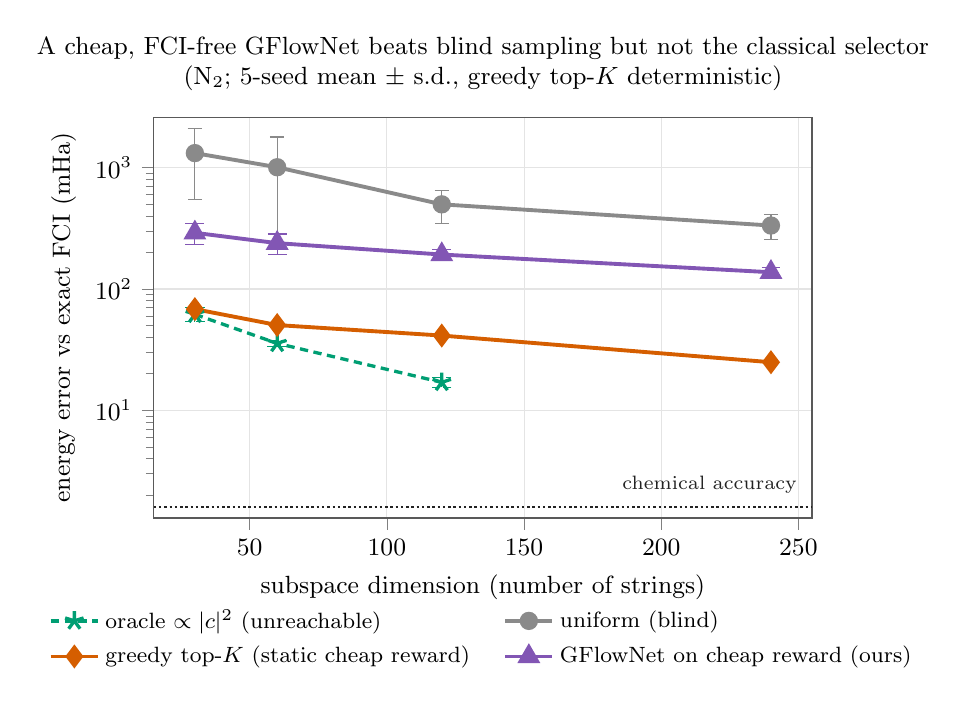
\begin{tikzpicture}
\begin{axis}[paperplot, width=0.82\linewidth, height=0.55\linewidth, ymode=log,
  xlabel={subspace dimension (number of strings)},
  ylabel={energy error vs exact FCI (mHa)},
  xmin=15, xmax=255, ymin=1.3, ymax=2600, xtick={50,100,150,200,250},
  title={A cheap, FCI-free GFlowNet beats blind sampling but not the classical selector\\(N$_2$; 5-seed mean $\pm$ s.d., greedy top-$K$ deterministic)},
  legend style={at={(0.5,-0.20)}, anchor=north, legend columns=2, /tikz/column 2/.style={column sep=10pt}},
  clip=false]
  \addplot[oiGreen, densely dashed, line width=1.2pt, mark=star, mark size=3.5pt, mark options={solid,fill=oiGreen},
    error bars/.cd, y dir=both, y explicit, error bar style={oiGreen}]
    coordinates {(30,61.8)+-(0,8.1) (60,35.6)+-(0,2.2) (120,17.0)+-(0,1.5)};
  \addlegendentry{oracle $\propto|c|^2$ (unreachable)}
  \addplot[oiGrey, line width=1.4pt, mark=*, mark size=2.6pt, mark options={fill=oiGrey},
    error bars/.cd, y dir=both, y explicit, error bar style={oiGrey}]
    coordinates {(30,1316.6)+-(0,768.6) (60,1006.9)+-(0,780.0) (120,498.0)+-(0,148.9) (240,333.1)+-(0,79.5)};
  \addlegendentry{uniform (blind)}
  \addplot[oiVerm, line width=1.4pt, mark=diamond*, mark size=3.2pt, mark options={fill=oiVerm}]
    coordinates {(30,68.2)(60,50.4)(120,41.3)(240,24.9)};
  \addlegendentry{greedy top-$K$ (static cheap reward)}
  \addplot[oiPurple, line width=1.4pt, mark=triangle*, mark size=3.4pt, mark options={fill=oiPurple},
    error bars/.cd, y dir=both, y explicit, error bar style={oiPurple}]
    coordinates {(30,290.0)+-(0,57.2) (60,238.5)+-(0,45.0) (120,192.1)+-(0,19.5) (240,137.3)+-(0,12.2)};
  \addlegendentry{GFlowNet on cheap reward (ours)}
  \draw[oiInk, densely dotted, line width=0.9pt] (axis cs:15,1.6) -- (axis cs:255,1.6);
  \node[oiInk, font=\scriptsize, anchor=south east] at (axis cs:253,1.72){chemical accuracy};
\end{axis}
\end{tikzpicture}
\caption{\textbf{Compactness under a cheap, FCI-free reward} (N$_2$, exact FCI; 5-seed mean~$\pm$~s.d.). Energy error vs subspace dimension for blind uniform sampling, deterministic top-$K$ selection by the static cheap Epstein--Nesbet reward, the GFlowNet trained on the same (tempered, $\beta{=}0.5$) cheap reward, and the exact $\propto|c|^2$ oracle. Averaged over five seeds, the ordering is unambiguous, and it is the ordering the paper's verdict predicts: the \emph{deterministic classical} greedy selector ($41.3$~mHa at $D{=}120$) beats the GFlowNet ($192\pm19$~mHa), which in turn beats only blind uniform sampling ($498\pm149$~mHa); the exact oracle ($17.0\pm1.5$~mHa) is out of reach of all three. The GFlowNet's diversity buys a large margin over blind sampling but none over the cheap classical selector it shares a reward with, consistent with the Spearman rank correlation of only ${\approx}0.64$ between that cheap reward and the true weights (\S\ref{sec:7}). An earlier single-seed version of this figure reported a near-oracle GFlowNet value; applying the multi-seed standard of \S\ref{sec:6}(v) to our own figure corrected it to the value shown, a concrete instance of why that standard is mandatory. The decisive comparison against the stronger \emph{iterative} heat-bath CI is Fig.~\ref{fig:hci}.}
\label{fig:compact}
\end{figure}


\subsection{A note on real-space neural wavefunctions}\label{sec:4-7}

For completeness and to forestall a common conflation, we distinguish the methods above from the real-space neural-wavefunction programme (FermiNet, PauliNet, Psiformer, and the emerging foundation models Neural Pfaffians and Orbformer) \cite{pfau2020,hermann2020,vonglehn2023,gao2024,foster2025}. These are variational Monte Carlo ans\"atze in continuous three-dimensional space, not determinant selectors in a fixed orbital basis; they are among the strongest classical methods for small strongly correlated molecules and thus appear in \S\ref{sec:5} as competitors. The discrete-orbital neural-network backflow of Liu and Clark reaches state-of-the-art molecular energies among them \cite{liuclark2024}; its optimized variant now matches heat-bath CI, ASCI, FCIQMC and DMRG and surpasses coupled cluster, making it the strongest single learned proposer to date \cite{liuclark2025} (a related neural ansatz reaches high accuracy with only a handful of Slater determinants \cite{fewdet2026}), and the programme is surveyed by \cite{hermann2023}. But these methods do not propose configurations for a diagonalization and are outside the loop this review concerns. The one bridge worth flagging is the discrete-basis autoregressive NQS (NAQS) \cite{barrett2022}, which \emph{does} sample determinants proportional to $|\psi|^2$ and is therefore the closest classical relative, and the most natural benchmark, for any learned determinant proposer, GFlowNet-based or otherwise.


\section{The critical assessment: does the quantum sampler, or its ML augmentation, beat classical selected CI?}\label{sec:5}

Every method in \S\ref{sec:4} is ultimately in service of an SQD subspace, and every SQD subspace inherits a single, unavoidable question. Because the final step is an exact diagonalization in a determinant subspace, SQD \emph{is} a selected configuration interaction whose determinants happen to be chosen by a quantum sampler. Its natural competitors are therefore the classical selected-CI heuristics --- and those are neither weak nor slow. A review that omitted this comparison would be advocacy, not assessment; we make it the centre of the paper.


\subsection{The classical baselines and the accuracy bar}\label{sec:5-1}

The relevant classical methods fall into two groups. The direct competitors are the classical determinant selectors: CIPSI, with its Epstein--Nesbet perturbative selection and extrapolation to the FCI limit \cite{huron1973,garniron2019,loos2024}; heat-bath CI (HCI) and its semistochastic form (SHCI), whose $|H_{ai}c_i|$ screening makes selection near-linear and which is generally the fastest route to sub-milli-hartree accuracy \cite{holmes2016,sharma2017}; and adaptive sampling CI (ASCI) \cite{tubman2016}. The best-in-class solvers for strong correlation are DMRG \cite{white1992,chan2002}, phaseless AFQMC \cite{zhangs2003}, full configuration-interaction quantum Monte Carlo \cite{booth2009}, and, for weak-to-moderate correlation, coupled cluster. Each of these baselines has a canonical, openly available implementation against which any claim can be reproduced (Dice for semistochastic heat-bath CI, Quantum Package for CIPSI, \texttt{block2} for DMRG, \texttt{ipie} for AFQMC, and NECI for FCIQMC, all interoperable through PySCF), and we take it as part of the standard below that a benchmark name the baseline code it was run against. The accuracy these methods agree on sets the bar any quantum result must clear to matter, and that bar is now quantitative: in the blind benzene ground-state challenge (a (30e,108o) space, a multi-method community effort), DMRG, AFQMC, FCIQMC, and SHCI concur on the correlation energy to a root-mean-square deviation of 1.3 mHa \cite{eriksen2020}, and the Simons hydrogen-chain benchmark reaches comparable cross-method concordance in the thermodynamic limit \cite{motta2017}. The same collaboration's transition-metal capstone (twenty first-principles methods on 3$d$ atoms, ions, and monoxides, with experiment-free reference values \cite{williams2020}) fixes the classical bar in exactly the strongly-correlated, 3$d$/iron--sulfur arena that SQD most wants to claim, and a curated open hierarchy of chemically decisive multireference systems (N$_2$, FeS, [2Fe-2S], U$_2$) has since been assembled to standardize such comparisons \cite{sundar2026}. The operative standard, then, is not ``reaches chemical accuracy'' but ``reaches the ${\sim}1.3$ mHa cross-method consensus at \emph{lower cost} than these methods, or in a regime where they all degrade.'' No SQD result has yet been measured against this bar and passed; indeed the largest systematic hardware benchmark to date (745 reactions on a superconducting processor) finds that SQD attains CCSD-level accuracy only after energy extrapolation, not directly \cite{raisuddin2025}.


\subsection{The critique literature}\label{sec:5-2}

Two peer-reviewed-track critiques frame the negative case. Reinholdt and co-workers, granting SQD an idealized noiseless sampler, show on N$_2$ and [2Fe-2S] (the very systems used to showcase the method) that its expansions are roughly an order of magnitude less compact than heat-bath CI (for [2Fe-2S], on the order of $5\times10^{4}$ determinants against heat-bath CI's ${\sim}4{,}300$ at matched accuracy), and that the coupon-collector cost to reach micro-hartree precision extrapolates to $\sim10^{14}$ samples; their conclusion is that QSCI ``falls behind more effective classical selected-CI heuristics'' \cite{reinholdt2025}. Gaberle and Jattana sharpen the claim for strongly correlated lattice models: the number of configurations required for a fixed accuracy grows \emph{exponentially with system size even under optimal, decreasing-probability inclusion}: even a \emph{perfect} sampler fails, so the limitation is intrinsic wavefunction delocalization, not a sampling artefact \cite{gaberle2026}. This second result is the more fundamental, and to date it has no proposed remedy.


\subsection{The 2026 dequantization}\label{sec:5-3}

The critique became concrete in 2026. Belagali and co-workers gave a polynomial-time classical algorithm for the energy of any single-layer local unitary cluster Jastrow circuit (the exact ansatz SQD samples), exploiting the fact that such a layer is a free-fermionic (matchgate) orbital rotation dressed by a low-rank diagonal-Coulomb (Jastrow) factor: the number--number Jastrow interactions are not themselves Gaussian, but at single-layer depth an extended-matchgate / fermionic-linear-optics treatment renders the energy classically tractable. The mechanism is specific: the Jastrow factor is diagonal in the occupation-number basis and low-rank, so the reduced density matrices needed for the energy collapse to Pfaffian-style evaluations over the free-fermionic vacuum rather than incurring the exponential cost a generic non-Gaussian layer would --- which is exactly why the single-layer result does not extend to deep, multi-layer circuits. They reproduced the flagship 77-qubit [4Fe-4S] experiment on a laptop in under a minute, finding, through classical circuit optimization, an energy \emph{below} the hardware result \cite{belagali2026}. The authors are careful that this is weak (energy) rather than strong (bitstring) simulation, leaving a formal gap; but as a statement about the specific published experiments it is decisive. Independently, a classical iterative refinement seeded from random determinants (TrimCI) reached the [4Fe-4S] ground state with on the order of $10^6$-fold fewer determinants than the quantum run \cite{zhangotten2025}, and the noise-and-recovery study of \S\ref{sec:3-2} showed random determinants plus classical recovery reproducing the accuracy \cite{vaquerosabater2026}. Taken together, these results locate the accuracy not in the quantum sampler but in the classical recovery-and-diagonalization back end. The trend has since consolidated. A fermionic-linear-optical (extended-matchgate) simulation not only reproduces the LUCJ circuit classically but \emph{improves} on the noisy-hardware SQD energy \cite{hassman2025}; this is unsurprising given device noise, the substantive point being that no quantum resource was needed, not that a new accuracy record was set. And, most tellingly, a bespoke classical eigenwalk solver from the same IBM authors who reported the 49-qubit advantage reportedly solves a subset of the instances underlying that claim classically \cite{chin2026}, so the advantage question is now partly self-refereed within a single group. In parallel, classical coupled-cluster and DMRG reached chemical accuracy on the FeMo-cofactor model long held up as the canonical quantum target \cite{zhai2026}, and transformer neural-network backflow surpassed DMRG on [2Fe-2S], the very iron--sulfur system SQD showcases \cite{ma2025}.


\subsection{The pro-quantum case, weighed on its own terms}\label{sec:5-4}

The defence is real but narrow. Hafid and co-workers prove that UCJ circuits can encode arbitrary instantaneous-quantum-polynomial (IQP) computations, so \emph{some} such circuits are classically hard to sample unless the polynomial hierarchy collapses \cite{hafid2025} --- a worst-case statement that does not describe the few-layer, chemically-structured LUCJ circuits actually run, which \S\ref{sec:5-3} shows are easy. Weaving and co-workers report time-evolved QSCI subspaces more than two hundred times more compact than a naive selected-CI criterion and ``comparable to HCI,'' but explicitly decline to claim a quantum advantage \cite{weaving2025}. The strongest experimental claim is Kirby and co-workers' 49-qubit sample-based Krylov result, reported to outperform classical sparse-ground-state solvers \cite{kirby2026} --- but on \emph{sparse-ground-state local Hamiltonians}, not general chemistry, a scope that must be stated precisely and whose classical rebuttals should be watched. The one genuinely open crack is depth: the dequantization proofs are for single-layer LUCJ, and whether deep, multi-layer LUCJ evades classical simulation is unresolved. It is the only place a future \emph{quantum-sampling-hardness} advantage could currently hide --- distinct from the noise-robustness effect of \S\ref{sec:7}, which a controlled test finds to be generic (shared by any constraint-respecting classical sampler, not a quantum edge), and from the multireference opening that same section leaves untested.


\subsection{Verdict}\label{sec:5-5}

The current state of the field, as of mid-2026, is that there is \emph{no reproducible, same-active-space demonstration that the SQD/QSCI quantum sampler beats SHCI, CIPSI, DMRG, or AFQMC (or even random determinants passed through classical recovery) on molecular electronic structure}, and that the flagship sampling circuits have been classically reproduced at the energy (weak-simulation) level. This is not a claim that SQD is useless: it is a genuinely useful, noise-tolerant, well-tooled workflow that has reached chemically relevant scale, and its configuration-recovery idea is a real contribution. It is a claim that the burden of proof for \emph{advantage} rests squarely on the quantum side, that this burden has not been met, and, the point of \S\ref{sec:6} and \S\ref{sec:7}, that meeting it, or ruling it out, requires a standard of benchmarking the field has not yet adopted. This verdict rests on the independent critique and dequantization literature above (not on any single computation of ours) and now coincides with independent macro-assessments of quantum advantage in electronic structure \cite{lee2023,gundlach2025,legeza2026}. Fig.~\ref{fig:hci} merely illustrates it on two FCI-verifiable systems, where iterative heat-bath CI --- grown from the Hartree--Fock reference by Epstein--Nesbet perturbative selection, each iteration re-scored against the current (increasingly correlated) wavefunction and never seeded from the exact solution --- reaches $0.6$~mHa on H$_2$O and $9.9$~mHa on stretched N$_2$, below both the noisy fused GFlowNet-SQD subspace and the noise-free cheap-reward GFlowNet subspace (Fig.~\ref{fig:compact}).


\begin{figure}[tb]
\centering
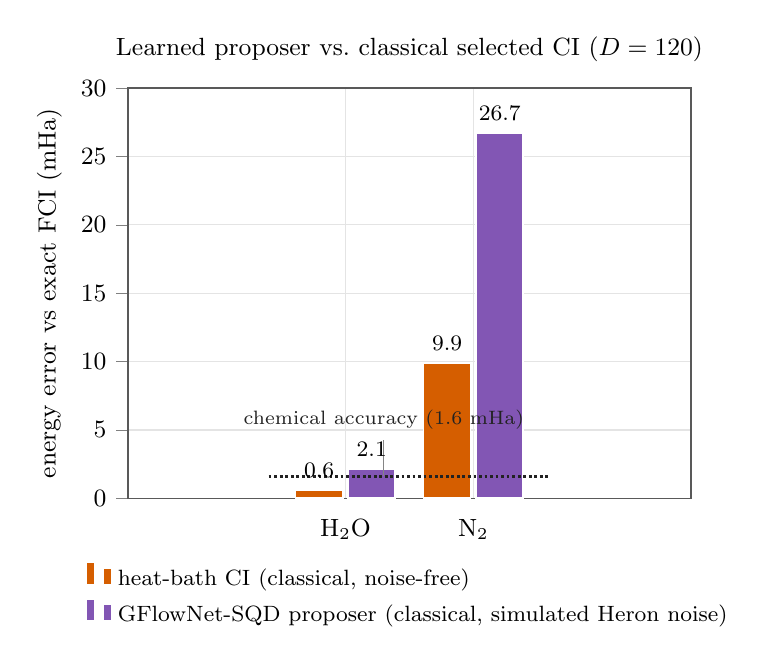
\begin{tikzpicture}
\begin{axis}[paperplot, ybar, width=0.72\linewidth, height=0.56\linewidth,
  bar width=17pt, ymin=0, ymax=30, xmin=-0.6, xmax=1.6,
  xtick={0,1}, xticklabels={H$_2$O, N$_2$}, xtick style={draw=none},
  ylabel={energy error vs exact FCI (mHa)}, ytick={0,5,10,15,20,25,30},
  title={Learned proposer vs.\ classical selected CI ($D=120$)},
  nodes near coords, nodes near coords style={font=\footnotesize\bfseries, /pgf/number format/fixed, /pgf/number format/precision=1, anchor=south, yshift=1pt},
  legend style={at={(0.5,-0.14)}, anchor=north, legend columns=1},
  enlarge x limits=0.5, clip=false]
  \addplot[fill=oiVerm, draw=white, line width=0.6pt] coordinates {(0,0.56) (1,9.9)}; \addlegendentry{heat-bath CI (classical, noise-free)}
  \addplot[fill=oiPurple, draw=white, line width=0.6pt] coordinates {(0,2.1) (1,26.7)}; \addlegendentry{GFlowNet-SQD proposer (classical, simulated Heron noise)}
  \draw[oiInk, densely dotted, line width=1pt] (axis cs:-0.6,1.6) -- (axis cs:1.6,1.6);
  \node[oiInk, font=\scriptsize, anchor=south] at (axis cs:0.30,4.35){chemical accuracy (1.6 mHa)};
  \draw[oiInk!55, line width=0.4pt] (axis cs:0.30,4.25) -- (axis cs:0.30,1.66);
\end{axis}
\end{tikzpicture}
\caption{\textbf{Classical selected CI versus a learned proposer at FCI-verifiable scale} ($D=120$; dotted line: chemical accuracy, $1.6$~mHa). Iterative heat-bath CI, grown from the Hartree--Fock reference by Epstein--Nesbet perturbative selection (never seeded from the exact wavefunction), reaches $0.6$~mHa on H$_2$O and $9.9$~mHa on stretched N$_2$, below the fused GFlowNet-SQD subspace built under simulated Heron noise ($2.1$ and $26.7$~mHa). This pits a noise-free classical selector against a noise-affected learned proposer, so it illustrates the gap at realistic conditions rather than isolating the proposer from the noise; the controlled, noise-matched test is the study \S\ref{sec:6} calls for.}
\label{fig:hci}
\end{figure}


\section{A standard for honest benchmarking}\label{sec:6}

The pattern that recurs across \S\ref{sec:5} is not that quantum methods were shown to fail, but that they were often not measured against the baselines that would settle the question. We therefore propose, and argue the field should adopt, a benchmarking standard with ten elements; we state it as a checklist because its value is in being applied uniformly. Systematic hardware benchmarking of SQD has recently begun \cite{raisuddin2025}; our emphasis differs in insisting on exact-FCI ground truth and an explicit dequantization baseline, and the checklist is exactly the protocol any defensible study of a learned proposer --- ours or others' --- would follow.

\textbf{(i) Exact ground truth at verifiable scale.} Claims about which determinants matter, and how compact a subspace is, are only meaningful where the exact answer is known. The controlled experiment should live in active spaces small enough for exact FCI (up to roughly a dozen orbitals) --- large enough for the coupon-collector effect to appear, small enough that every energy is an error against truth, not against another approximation. This is a deliberate inversion of the ``largest active space'' instinct: the point is not scale but falsifiability.

\textbf{(ii) The strong classical baseline, not a straw man.} The comparison must be against iterative heat-bath / semistochastic CI bootstrapped from the correlated wavefunction --- and, following \S\ref{sec:5-3}, against the two baselines the field has repeatedly found decisive: random determinants passed through the classical recovery loop, and the classical simulation of the sampling circuit itself. A method that beats uniform sampling but not SHCI has demonstrated nothing about quantum value.

\textbf{(iii) A dequantization baseline.} Given \cite{belagali2026}, any hardware claim should report whether the sampling circuit is classically simulable at the depth used, and if so, the energy that classical simulation attains. This is now as basic a control as reporting the classical FCI reference, and it has four independent routes the strongest studies report against wherever they apply: fermionic-linear-optical (matchgate) simulation \cite{belagali2026,hassman2025}, sparse guided eigenwalks \cite{chin2026}, Pauli propagation \cite{shrikhande2025}, and direct tensor-network (matrix-product-state) contraction of the circuit --- the last two being the depth-truncable routes that most directly probe the multi-layer-LUCJ crack of \S\ref{sec:5-4}.

\textbf{(iv) Full cost accounting in the currency that is scarce.} The scarce resource is quantum measurement (shots = QPU time), and the honest axis is energy error versus shots, or versus subspace dimension at matched classical diagonalization cost --- not energy error versus wall-clock on incomparable hardware. Reporting the shot budget honestly also surfaces the early saturation of \S\ref{sec:3-3}.

\textbf{(v) Statistical error bars.} Sampling is stochastic and neural proposers are seed-dependent; a single run is an anecdote. Multi-seed means and standard deviations, and a significance statement on any claimed separation, should be mandatory. In our own work a single-seed run of the compactness study reported a \emph{near-oracle} generative value; the five-seed standard corrected it to one an order of magnitude above the oracle it had appeared to match (Fig.~\ref{fig:compact}). And with only five seeds even a real separation is fragile: the sharpest distribution-free statement is a sign test (floor $p{=}0.0625$ at $n{=}5$), so a controlled sweep should carry many seeds and report the test, not a parametric $\sigma$ extrapolated past what five points resolve (Fig.~\ref{fig:crossover}). Both are cautionary instances of exactly this point.

\textbf{(vi) Backend-calibrated, asymmetric noise.} Because SQD's noise sensitivity runs through particle-number-violating readout errors (\S\ref{sec:3-2}), a credible noise model must be backend-calibrated and must include the $T_1$-driven asymmetry of readout, which symmetric bit-flip models understate; and the analysis should include an ablation isolating that asymmetry. A readout-only model will, in turn, be criticized where gate errors dominate, so the strongest studies will move toward full noisy-circuit simulation or a confirmatory hardware point.

\textbf{(vii) Convergence of the reduction to the model problem.} Every SQD number is a claim about a chosen active space in a chosen basis; the benchmark should report active-space, basis-set, and orbital-choice (natural- versus canonical-orbital) convergence, so that an apparent advantage is not an artefact of a fortunate truncation.

\textbf{(viii) Energy differences and properties, not only total energies.} Chemistry is decided by relative quantities --- barriers, spin gaps, dissociation energies --- and a method can reach a good total energy while misranking the differences that matter; a benchmark should report at least one chemically decisive energy difference, not a single total energy.

\textbf{(ix) More than one geometry.} A single-point win can be a coincidence of the reference; several geometries along a dissociation or reaction coordinate test whether the advantage is systematic, and are the natural setting for the amortization question of \S7.

\textbf{(x) Pre-registered, commensurate total-resource accounting.} Beyond the shot axis of (iv), the true total cost is quantum and classical together --- QPU-seconds reported alongside the classical node-hours of the diagonalization and recovery, in the commensurate-resource spirit of \cite{raisuddin2025} --- and the seed count and significance threshold of (v) should be fixed before the runs, not chosen after.

We contend that a study meeting all ten is publishable and valuable \emph{whatever its result} --- a rigorous negative result that maps where a generative or quantum proposer does and does not help is, in a field this contested and this prone to under-benchmarked demonstrations, more useful than another hopeful positive that a strong baseline would deflate.


\section{Outlook: where generative and quantum methods retain a defensible advantage}\label{sec:7}


\begin{figure*}[tb]
\centering
\begin{tikzpicture}[font=\sffamily,
  panel/.style={rounded corners=4pt, minimum width=5.4cm, minimum height=7.4cm, line width=1pt, anchor=north west},
  hdr/.style={font=\bfseries, align=center},
  chip/.style={rounded corners=6pt, text=white, font=\footnotesize\bfseries, inner sep=3pt, minimum height=0.5cm},
  body/.style={anchor=north west, align=left, font=\scriptsize, text width=4.9cm, inner sep=0pt},
  ital/.style={anchor=south west, align=left, font=\scriptsize\itshape, text width=4.9cm},
]
\definecolor{zRedF}{HTML}{FBECEC}\definecolor{zRedS}{HTML}{D55E00}\definecolor{zRedT}{HTML}{9C3D00}
\definecolor{zOrgF}{HTML}{FDF2E0}\definecolor{zOrgS}{HTML}{E69F00}\definecolor{zOrgT}{HTML}{9A6A00}
\definecolor{zGrnF}{HTML}{E7F6F0}\definecolor{zGrnS}{HTML}{009E73}\definecolor{zGrnT}{HTML}{00795A}
% title
\node[anchor=north west, font=\large\bfseries, text=black] at (0,0.5) {Where a quantum or generative advantage can, and cannot, live};
\node[anchor=north west, font=\small, text=black!55, text width=17cm] at (0,-0.15)
  {The structure that makes SQD classically \emph{verifiable} is the structure that makes it classically \emph{constructible}. Advantage survives only where that equivalence breaks.};
% ---- panels ----
\node[panel, fill=zRedF, draw=zRedS] (P1) at (0,-1.7) {};
\node[panel, fill=zOrgF, draw=zOrgS] (P2) at (5.9,-1.7) {};
\node[panel, fill=zGrnF, draw=zGrnS] (P3) at (11.8,-1.7) {};
% headers + chips
\node[hdr, text=zRedT] at ([yshift=-6mm]P1.north) {Classically verifiable\\\& simulable};
\node[hdr, text=zOrgT] at ([yshift=-6mm]P2.north) {Classical signal\\degrades};
\node[hdr, text=zGrnT] at ([yshift=-6mm]P3.north) {Provably hard\\classically};
\node[chip, fill=zRedS] at ([yshift=-19mm]P1.north) {CLASSICAL WINS};
\node[chip, fill=zOrgS] at ([yshift=-19mm]P2.north) {OPEN / CONDITIONAL};
\node[chip, fill=zGrnS] at ([yshift=-19mm]P3.north) {ADVANTAGE = THEOREM};
% bodies
\node[body, text=black!80] at ([xshift=3mm,yshift=-23mm]P1.north west)
  {\textbf{Task:} molecular ground-state SQD\\[2pt]
   $\bullet$ SHCI / CIPSI / DMRG / AFQMC reach the ${\sim}$1.3 mHa consensus at lower cost\\[1pt]
   $\bullet$ LUCJ circuits dequantized on a laptop; random+recovery matches\\[1pt]
   $\bullet$ exponential even for a perfect sampler in delocalized states};
\node[ital, text=zRedT] at ([xshift=3mm,yshift=5mm]P1.south west) {The generative advantage is dequantized along with the sampler.};
\node[body, text=black!80] at ([xshift=3mm,yshift=-23mm]P2.north west)
  {\textbf{Where the cheap prior fails:}\\[2pt]
   $\bullet$ high noise $\rightarrow$ starved valid-shot budget; symmetry-valid generators waste nothing {\footnotesize\itshape(demonstrated, but generic --- not a quantum edge)}\\[1pt]
   $\bullet$ strong multireference $\rightarrow$ HF-based perturbative ranking misfires {\footnotesize\itshape(open; untested)}\\[1pt]
   $\bullet$ amortization across a PES / chemical series (train once)};
\node[ital, text=zOrgT] at ([xshift=3mm,yshift=5mm]P2.south west) {The empirical target of \S\ref{sec:6}--\S\ref{sec:7} (GFlowNet).};
\node[body, text=black!80] at ([xshift=3mm,yshift=-23mm]P3.north west)
  {\textbf{Task:} learning from experiments\\[2pt]
   $\bullet$ two-copy / quantum-memory learning: exponential separation, \textbf{unconditional} (a theorem, not a conjecture)\\[1pt]
   $\bullet$ cannot be dequantized\\[2pt]
   \textbf{Caveats:} tasks are contrived; fragile on NISQ hardware; useful reach = device characterization};
\node[ital, text=zGrnT] at ([xshift=3mm,yshift=5mm]P3.south west) {The highest-value open bridge to chemistry.};
% ---- gradient arrow ----
\shade[left color=zRedS, right color=zGrnS, middle color=zOrgS, rounded corners=5pt] (0,-9.8) rectangle (16.6,-9.3);
\draw[-{Stealth[length=4mm,width=4mm]}, line width=1.2pt, black!80] (0,-9.55) -- (17.2,-9.55);
\node[anchor=north west, font=\small\bfseries, text=black!75] at (0,-9.95) {cheap classical construction \& verification};
\node[anchor=north east, font=\small\bfseries, text=black!75] at (16.6,-9.95) {classical construction provably expensive};
\node[anchor=north, font=\small\bfseries, text=black] at (8.3,-10.5) {$\rightarrow$\ \ aim generative \& quantum methods where classical proof is NOT cheap\ \ $\rightarrow$};
\end{tikzpicture}
\caption{\textbf{The advantage landscape of \S5--\S7.} The structure that makes SQD classically \emph{verifiable} is the structure that makes it classically \emph{constructible}; advantage survives only where that equivalence breaks. Colour-blind-safe (Okabe--Ito) palette; zones are also distinguished by header text and verdict chips, not colour alone.}
\label{fig:landscape}
\end{figure*}

The verdict of \S\ref{sec:5} is easy to read as a counsel of despair; we read it instead as a map. The reason classical selected CI wins the SQD contest, on the systems studied, is structural: SQD's task is \emph{classically verifiable}, and, empirically on molecular systems, the same structure that lets one check a subspace (a projected Hamiltonian one can diagonalize) also makes a cheap classical \emph{importance heuristic} available with which to construct it; the dequantization of \S\ref{sec:5-3} is the extreme statement of the same fact, that even the sampler is classically reproducible. (This is an observation about the available classical signal, not a general implication of verifiability: verifiability alone need not imply cheap constructibility, as the P-versus-NP gap makes plain.) There is little quantum edge to be had where such a cheap classical construction happens to exist.

This is not a wall but a compass (Fig.~\ref{fig:landscape}): it says to aim generative and quantum methods at the regimes where a strong classical baseline provably \emph{cannot} be cheap. This converts the compass from a metaphor into a falsifiable prediction the standard of \S\ref{sec:6} can test: if the locus of advantage is exactly where the cheap importance signal misranks the truly important determinants, then any genuine generative or quantum advantage on molecular electronic structure should appear first, and preferentially, where the \emph{rank correlation between the cheap prior (e.g. the Epstein--Nesbet coefficient) and the exact CI weights degrades most}. That rank correlation is directly measurable at FCI-verifiable scale, and our own minimal computational experiment both confirms it is imperfect and shows it behaving as a monotone multireference coordinate. Over the 792 $\alpha$-strings of the N$_2$(10e,12o) active space, the Spearman correlation between the cheap Epstein--Nesbet reward and the exact $|c|^2$ is $\rho{\approx}0.64$ at $R=2.0$~\AA{}; more tellingly, it \emph{degrades monotonically as the wavefunction becomes more multireference}, falling from $\rho{=}0.72$ near equilibrium ($R=1.1$~\AA{}: Hartree--Fock weight $0.93$, frontier natural-orbital occupations $1.95/0.06$) through $0.64$ at $R=2.0$~\AA{} (HF weight $0.34$, occupations $1.32/0.68$) to $0.60$ at $R=2.5$~\AA{} (HF weight $0.12$, occupations $1.08/0.92$, the sum of fractional occupancy rising from $0.29$ to $5.10$). This is that coordinate, measured (Fig.~\ref{fig:orderparam}): the scalar declines monotonically where static correlation grows --- though it is the Hartree--Fock weight ($0.93\to0.12$) and the natural-orbital occupations, not $\rho$ itself, that genuinely collapse. Notably $\rho$ stays ${\approx}0.60$-informative even at maximal static correlation, so the cheap prior is \emph{degraded, not destroyed} by multireference character (consistent with Fig.~\ref{fig:compact}, where deterministic top-$K$ on that prior still beats the GFlowNet). Two caveats a specialist will demand: by the Slater--Condon rules the reward is exactly zero for the ${\sim}69\%$ of $\alpha$-strings that are triple-or-higher excitations of Hartree--Fock, so $\rho$ over all strings is a blunt, tie-laden statistic; and its precise value carries a small gauge dependence from the arbitrary rotation within the degenerate $\pi$ shells. We therefore rely on the monotone \emph{trend}, not the absolute value, and propose $\rho$ as a low-cost coordinate for where to look --- computable system by system before any hardware is run. A method that helps where the prior already ranks well would falsify the picture; one that helps only as $\rho$ degrades would confirm it. Three such regimes are visible.

\begin{figure}[tb]
\centering
\begin{tikzpicture}
\begin{groupplot}[group style={group size=2 by 1, horizontal sep=1.7cm}, paperplot,
  width=0.44\linewidth, height=0.40\linewidth, xmin=1.0, xmax=2.6, xtick={1.1,1.4,1.7,2.0,2.3,2.5}]
\nextgroupplot[xlabel={N$_2$ bond length $R$ (\AA)}, ylabel={Spearman $\rho$ (order parameter)},
  ymin=0.55, ymax=0.76, title={the cheap prior degrades\dots}]
  \addplot[oiBlue, line width=1.4pt, mark=*, mark size=2.7pt, mark options={fill=oiBlue,draw=white}]
    table[x=R,y=spearman]{orderparam.dat};
  \node[font=\bfseries\large, anchor=south east] at (rel axis cs:-0.20,1.0){a};
\nextgroupplot[xlabel={N$_2$ bond length $R$ (\AA)}, ylabel={multireference character},
  ymin=0, ymax=1, title={\dots where static correlation grows},
  legend style={at={(0.5,-0.32)}, anchor=north, legend columns=1, draw=none, fill=none, font=\footnotesize}]
  \addplot[oiVerm, line width=1.4pt, mark=square*, mark size=2.5pt, mark options={fill=oiVerm,draw=white}]
    table[x=R,y=mrweight]{orderparam.dat}; \addlegendentry{$1-w_{\mathrm{HF}}$ (weight off Hartree--Fock)}
  \addplot[oiOrange, line width=1.4pt, densely dashed, mark=triangle*, mark size=3.2pt, mark options={fill=oiOrange,draw=white,solid}]
    table[x=R,y=lumo_noon]{orderparam.dat}; \addlegendentry{LUMO natural-orbital occupation}
  \node[font=\bfseries\large, anchor=south east] at (rel axis cs:-0.20,1.0){b};
\end{groupplot}
\end{tikzpicture}
\caption{\textbf{The cheap prior degrades with multireference character (N$_2$ across geometries).} \emph{(a)} The Spearman rank correlation between the cheap Epstein--Nesbet reward and the exact FCI $|c|^2$ (over all 792 $\alpha$-strings) falls monotonically as the triple bond stretches, from $\rho{=}0.72$ near equilibrium to $0.60$ at $R{=}2.5$~\AA. \emph{(b)} Over the same interval the wavefunction becomes strongly multireference: the weight carried by determinants \emph{other} than Hartree--Fock rises from $0.07$ to $0.88$, and the frontier natural-orbital occupations open from the closed-shell $2/0$ toward the dissociation limit $1/1$ (LUMO occupation $0.06\to0.92$). The cheap classical importance signal that makes an SQD subspace \emph{verifiable} degrades exactly where static correlation makes it harder to \emph{construct} --- so the single scalar $\rho$ predicts, before any hardware is run, where a learned or quantum proposer has room to help.}
\label{fig:orderparam}
\end{figure}

\textbf{Noise-limited recovery, and a controlled test of the multireference hypothesis.} Within SQD itself the classical selectors win because a cheap classical importance signal (a Hartree--Fock-referenced perturbative estimate) is available and accurate. The one regime where a learned proposer has room is high noise: as the valid-shot budget is starved, a generator that emits only symmetry-valid configurations \emph{by construction} wastes nothing, whereas the classical control loses a growing fraction of its samples to particle-number violation. The fair baseline here is no straw man --- it is the noise-robust recovery loop of \S\ref{sec:5-3} itself (S-CORE plus the cheap prior that already reproduces the accuracy), so any generative gain is measured \emph{beyond} that classical recovery; and because the classical learned rankers of \S\ref{sec:4-4} already contest, and on Cr$_2$ reportedly beat, SHCI with no quantum resource, the live question is the \emph{incremental} value of the quantum samples, not of learning over perturbation theory. Our first reading of this gain was that it is \emph{multireference-specific}: that it should appear only where a single-reference prior misranks the important determinants. \emph{A controlled experiment refutes that reading.} We ran the noise sweep along the N$_2$ dissociation coordinate at fixed active space (10e,12o), so that only multireference character varies --- from near-single-reference at $R{=}1.1$~\AA{} (HF weight $0.93$, $\rho{=}0.72$) to strongly multireference at $R{=}2.5$~\AA{} (HF weight $0.12$, $\rho{=}0.60$) --- with molecule, electron count, and Hilbert dimension held \emph{constant} (Fig.~\ref{fig:crossover}). The crossover is \emph{universal}: at $3\times$ Heron noise the generative proposer wins at \emph{every} geometry, by $+10$ to $+21$~mHa and positive in all five seeds at each point, including the near-single-reference $R{=}1.1$ case. What multireference character controls is instead the \emph{zero-noise} baseline: the classical advantage is largest at the stretched, strongly multireference geometries ($-6.9$ and $-7.9$~mHa at $R{=}2.0$ and $2.5$~\AA) and smaller near equilibrium ($-1.9$~mHa at $R{=}1.1$; the intermediate $R{=}1.7$ point is statistically null, $-0.2\pm1.8$~mHa, $t_4{=}-0.3$, so the endpoint trend toward a deeper classical advantage with multireference character is noisy rather than strictly monotone). Either way it is the opposite of a generative opening. The two axes are decoupled: \emph{valid-shot starvation}, not multireference character, drives the crossover, and it does so across the whole dissociation curve.

This also exposes the confound in a naive stretched-N$_2$-versus-equilibrium-H$_2$O contrast (single-reference H$_2$O shows no \emph{significant} crossover: $-2.9\pm1.0$~mHa at $2\times$, and its nominal sign-flip at $3\times$, $+1.4\pm4.5$~mHa, is consistent with zero): at fixed $D{=}120$, H$_2$O covers $24\%$ of its 495-string space against N$_2$'s $15\%$ of 792, so its classical fill is simply more complete --- a coverage effect, not a chemistry effect, and not the multireference-specificity we first inferred from it.

The honest conclusion is narrower and, we think, more useful than our first one: the only generative advantage we can demonstrate is a \emph{noise-robustness} effect (valid-by-construction sampling under shot starvation), available in principle across chemistry rather than confined to the multireference regime --- and it is \emph{not} a quantum or chemistry advantage, since any constraint-respecting classical sampler shares the mechanism. The multireference \emph{prediction} of the order parameter above is left \emph{untested} by this experiment, which varies noise rather than prior quality at fixed noise; cleanly separating those two axes is the controlled study \S\ref{sec:6} still calls for (e.g.\ on Cr$_2$ or a metal dimer). Two statistical caveats belong with the result: with five seeds the sharpest distribution-free statement is that all five agree in sign (a sign-flip test floors at $p{=}0.0625$; the parametric $t_4$ values we quote are reproducibility diagnostics, not discovery significances), and each per-geometry test certifies seed reproducibility, not generalization across chemical space. That a controlled test of our own hypothesis returns a partial negative is, by the standard of \S\ref{sec:6}, exactly the kind of result this field needs more of.


\begin{figure}[tb]
\centering
\begin{tikzpicture}
\begin{axis}[paperplot, width=0.82\linewidth, height=0.54\linewidth,
  xlabel={N$_2$ bond length $R$ (\AA)\ \ [more multireference $\rightarrow$]},
  ylabel={gap $E_{\mathrm{ibm+cheap}}-E_{\mathrm{gfn}}$\,\,(mHa)},
  xmin=1.0, xmax=2.6, ymin=-17, ymax=35, xtick={1.1,1.7,2.0,2.5}, xticklabels={1.1,1.7,2.0,2.5},
  title={Controlled single-molecule test: the crossover is universal\\across N$_2$ dissociation --- driven by noise, not multireference},
  legend style={at={(0.5,-0.24)}, anchor=north, legend columns=2, draw=none, fill=none, /tikz/every even column/.append style={column sep=12pt}}, clip=false]
  \addplot[draw=none, fill=oiGreen, fill opacity=0.06, forget plot] coordinates {(1.0,0)(2.6,0)(2.6,35)(1.0,35)}\closedcycle;
  \addplot[draw=none, fill=oiVerm, fill opacity=0.06, forget plot] coordinates {(1.0,-17)(2.6,-17)(2.6,0)(1.0,0)}\closedcycle;
  \draw[oiInk, line width=0.7pt] (axis cs:1.0,0) -- (axis cs:2.6,0);
  \addplot[oiBlue, line width=1.4pt, mark=square*, mark size=3pt, mark options={fill=oiBlue, draw=white, line width=0.6pt},
    error bars/.cd, y dir=both, y explicit, error bar style={oiBlue, line width=1pt}, error mark options={rotate=90, mark size=3pt}]
    table[x=R, y=gap3, y error=gap3sd]{ladder.dat};
  \addlegendentry{$3\times$ Heron noise}
  \addplot[oiOrange, line width=1.4pt, densely dashed, mark=triangle*, mark size=3.6pt, mark options={fill=oiOrange, draw=white, line width=0.5pt, solid},
    error bars/.cd, y dir=both, y explicit, error bar style={oiOrange, line width=1pt}, error mark options={rotate=90, mark size=3pt}]
    table[x=R, y=gap0, y error=gap0sd]{ladder.dat};
  \addlegendentry{no noise ($0\times$)}
  \node[oiGreen, font=\small\bfseries, anchor=west] at (axis cs:1.04,32){GFlowNet better};
  \node[oiVerm, font=\small\bfseries, anchor=west] at (axis cs:1.04,-14){classical control better};
\end{axis}
\end{tikzpicture}
\caption{\textbf{A controlled single-molecule test refutes multireference-specificity of the noise crossover.} Classical-minus-generative energy-error gap for N$_2$ at fixed active space (10e,12o), swept along the dissociation coordinate so that \emph{only} multireference character varies (HF weight $0.93\to0.12$ as $R{=}1.1\to2.5$~\AA), with molecule, electron count, and Hilbert dimension held constant; mean~$\pm$~s.d.\ over five seeds at $D{=}120$. \emph{At $3\times$ Heron noise} (blue) the constraint-respecting generative proposer wins at \emph{every} geometry ($+10$ to $+21$~mHa, positive in all five seeds at every geometry), including near-single-reference $R{=}1.1$ --- so the crossover is driven by valid-shot starvation ($\sim$51\% lost at $3\times$, essentially constant across $R$), \emph{not} by multireference character. \emph{At zero noise} (orange) the classical control wins at three of the four geometries --- deepest at the strongly multireference $R{=}2.0,2.5$ points ($-6.9$, $-7.9$~mHa) and statistically null at the intermediate $R{=}1.7$ ($-0.2\pm1.8$~mHa, $t_4{=}-0.3$) --- the opposite of a generative opening. The two effects are decoupled. With five seeds the distribution-free significance floors at $p{=}0.0625$ (all seeds agree in sign); the parametric $t_4$ is a reproducibility diagnostic only. The apparent multireference-specificity of an earlier stretched-N$_2$-versus-equilibrium-H$_2$O contrast was a subspace-coverage confound ($24\%$ vs $15\%$ of the target space at fixed $D$; \S\ref{sec:7}), which this single-molecule design removes.}
\label{fig:crossover}
\end{figure}

\textbf{Amortization across chemical space.} A learned proposer offers something a per-instance classical selector does not: amortization. A model conditioned on molecular geometry and trained once can, in principle, generate compact subspaces across an entire dissociation curve or chemical series without re-running an expensive selection at each point --- the value proposition of the foundation-wavefunction programme \cite{foster2025}, transposed to the determinant-selection setting. Here the metric is not accuracy at one geometry but total cost across many, and it is a genuinely open, and genuinely ML-flavoured, question whether amortization beats re-running SHCI per point.

\textbf{Learning from experiments: where the advantage is a theorem.} The deepest reason for optimism lies just outside the SQD loop, and it inverts the logic of \S\ref{sec:5} exactly. The one place in this landscape with an \emph{unconditional, information-theoretic} quantum advantage is the quantum-data-native task of learning properties of an unknown quantum state or process: a learner with quantum memory that measures two coherent copies jointly needs exponentially fewer experiments than any single-copy strategy, a separation proved without complexity assumptions \cite{chen2021} and demonstrated on superconducting and photonic hardware \cite{huang2022,liuphotonic2025}, and surveyed among the field's few unconditional advantages by \cite{huang2025}. Unlike SQD, this advantage cannot be dequantized, because its classical lower bound is a theorem, not a conjecture about circuit structure. This suggests a reorganizing principle for the enterprise as a whole: candidate quantum advantages should be sorted not by their promised magnitude but by the \emph{type} of their classical lower bound. Those resting on a complexity-theoretic conjecture (the presumed hardness of sampling a particular circuit family) are perpetually one clever classical algorithm away from collapse, as SQD's own two-year arc from flagship experiment to laptop reproduction (\S\ref{sec:5-3}) attests; those resting on an unconditional, information-theoretic separation are not, because no future algorithm can close a gap that is already a theorem. A field repeatedly surprised by dequantization would do well to spend its scarce hardware where the lower bound is a theorem, and to treat conjecture-backed advantages as demonstrations of scale, not of separation, until proven otherwise. Its caveats are equally sharp and belong in any forward-looking account: the demonstrated-advantage \emph{tasks} (predicting Pauli expectations, purity, and random-channel characteristic functions) are information-theoretically natural but scientifically contrived; the advantage is fragile on superconducting hardware, degrading under the depolarizing noise of a heavy-hex device \cite{cotler2025} to the reduced, mitigation-propped separation IBM has actually measured \cite{seif2024}; and the one \emph{useful} application delivered with rigorous backing is the characterization of quantum devices themselves. The bridge from this provable-but-contrived frontier to genuinely useful chemistry is, we argue, the highest-value open problem adjacent to the subfield, and the natural destination for the generative machinery reviewed here. That bridge might be built by learning a device's effective error model (as machine-learning quantum error mitigation already does at utility scale \cite{liao2024}) to improve an SQD estimator, or by learning the properties of a molecular state prepared on hardware.


\section{Conclusions and open problems}\label{sec:8}

Machine learning entered sample-based quantum diagonalization for a sound reason (the configuration-recovery step is a selection-and-denoising problem that a learned model should do better than an occupancy-weighted heuristic), and in two years has produced a rich ecosystem of restricted Boltzmann machines, neural-quantum-state proposers, classifiers, ranking models, and generative circuit designers. This review has organized that ecosystem, mapped its methods and open-source tooling, and, most importantly, insisted on holding it to the question it exists to answer. That verdict, stated in \S\ref{sec:5-5}, is at present a negative one: no verifiable-scale demonstration that the quantum sampler or its machine-learning augmentation beats classical selected configuration interaction on molecular electronic structure, and flagship sampling circuits now classically reproducible at the energy (weak-simulation) level. We have argued that it is a compass rather than a counsel of futility: it points generative methods toward the noise-limited and multireference regimes where the cheap classical signal fails, toward amortization across chemical space, and, as an adjacent horizon, toward the quantum-data-native learning tasks where the advantage is provable but not yet connected to useful chemistry. A controlled FCI-exact experiment already sharpens the first of these into a candid partial negative: the prior's rank correlation with the truth declines with multireference character (a usable coordinate), but the generative noise-crossover turns out to be a generic shot-starvation effect, present across the N$_2$ dissociation curve rather than multireference-specific (\S\ref{sec:7}).

Four open problems structure the road ahead. First, the \emph{intrinsic-delocalization} barrier of \cite{gaberle2026} (that some strongly correlated ground states require exponentially many configurations even under a perfect sampler) has no proposed remedy and may be fundamental. Second, the \emph{depth} question: whether deep, multi-layer LUCJ circuits evade the classical simulability that \cite{belagali2026} proved for the single-layer case is the one place a \emph{quantum-sampling-hardness} advantage could still live, and settling it is urgent. We flag a structural worry worth confronting rather than postponing. The VQE programme collapsed when it emerged that the conditions letting a circuit avoid barren plateaus tend also to render it classically simulable \cite{cerezo2025}; SQD may face an isomorphic dichotomy in a different dialect, since the shallow, structured, low-entanglement circuits whose samples are noise-tolerant and amenable to configuration recovery are precisely those most exposed to matchgate-style dequantization \cite{belagali2026}, while the depth that would defeat classical simulation may also be the depth at which readout noise and the coupon-collector tail (\S\ref{sec:3-1}) overwhelm the loop. Whether a usable corridor exists between these two failure modes is, we conjecture, the question on which a near-term \emph{chemistry} advantage for SQD ultimately rests, and it is one the field has the tools to settle. Third, the \emph{useful-target} gap in learning-from-experiments (bridging provable-but-contrived tasks to science anyone needs) is the highest-value problem adjacent to the field. Fourth, and most immediately actionable, the \emph{GFlowNet gap}: the one generative paradigm built for diverse, reward-proportional sampling over exponential discrete spaces has not been applied to determinant selection, and whether it helps, measured (per \S\ref{sec:6}) against exact ground truth and strong classical baselines, is a clean, falsifiable, and currently unclaimed question. We have tried to write the review such that its most useful legacy would be not a catalogue but a standard: that the next claim in this field, positive or negative, arrives with exact ground truth, strong and dequantization baselines, full cost accounting, and error bars, so that the field can, at last, know what it knows.

\emph{Limitations of this review.} This survey is a snapshot of a subfield that is expanding on a timescale of weeks; a substantial fraction of the primary literature we cite is preprint and not yet peer-reviewed. We have verified the authors, venues, and arXiv/DOI identifiers of the works most central to the verdict, but preprint metadata can still shift, and readers should confirm against the published versions of record. Our coverage extends to mid-2026 and will inevitably miss work that appears between writing and publication, including, very possibly, the first application of a generative-flow network to determinant selection whose absence we here record. We have tried to make the review robust to that churn by organizing it around durable questions (compactness, verifiability, the locus of advantage) and a benchmarking standard, rather than around any single result. Finally, a positional disclosure: the author is actively developing the generative-flow-network proposer whose absence this review documents, and the standard of \S\ref{sec:6} is the protocol that study is intended to meet. The GFlowNet gap is therefore presented as an open, falsifiable question (one that forthcoming study may well answer in the negative) rather than a solved one, and the \S\ref{sec:5} verdict rests on the independent literature rather than on the author's own illustrative figures.


\section*{Data and code availability}
\small
Every quantitative result we compute ourselves in this review --- as distinct from the numbers we quote from the cited literature --- is reproduced from executable code in the companion computational
notebook \texttt{GFlowNet\_SQD\_calculations.ipynb}, which runs in Google Colab or any Python~$\ge$3.10 with
\texttt{pyscf}, \texttt{torch}, \texttt{scipy}, and \texttt{matplotlib}. The notebook and calculation scripts regenerate, from first
principles and with fixed random seeds, the exact FCI reference of the systems in Fig.~\ref{fig:system}, the coupon-collector
statistics of \S\ref{sec:3}, the S-CORE recovery of \S\ref{sec:3-2}, the Epstein--Nesbet reward and GFlowNet compactness study of
\S\ref{sec:4}, the natural-orbital occupations and order-parameter sweep (Fig.~\ref{fig:orderparam}) together with the controlled single-molecule noise-crossover sweep (Fig.~\ref{fig:crossover}) of \S\ref{sec:7}, and the heat-bath-CI decisive test of \S\ref{sec:5}. The complete code --- the notebook,
the calculation scripts behind every reported number, one script per figure, the generated figures, and the
Docker build environments --- is openly available (MIT license) at \url{https://github.com/nicolasbonilla/ml-for-sqd-review},
with a one-click Google~Colab entry point and every notebook cell and figure rendered inline in the browser.
Fig.~\ref{fig:loop} was produced as native vector graphics; Fig.~\ref{fig:system} combines vector molecular-orbital diagrams with high-resolution ($\ge$300~dpi at print size) ray-traced (PyMOL) isosurface renders, and all figure sources are available with the code. No proprietary data or
hardware access is required to reproduce any figure or table; all ``real-noise'' results use local,
backend-calibrated noise models (\texttt{FakeTorino}, IBM Heron~r1).

\section*{Author contributions}
\small
N.B.V.\ conceived the review, performed the literature synthesis, designed and ran all computational
experiments, produced the figures, and wrote the manuscript.

\section*{Competing interests}
\small
The author declares no competing financial interests. As a non-financial interest, the author is developing a generative-flow-network determinant proposer for SQD of the kind this review identifies as a methodological gap (\S\ref{sec:4-6}, \S\ref{sec:8}). The review documents that gap from the published literature and rests its central verdict on independent results, not on the author's own illustrative computations; this disclosure is made in the interest of full transparency.

\section*{Acknowledgements}
\small
The author thanks the IBM Quantum and Qiskit communities and the organizers of the Qiskit Global Summer School,
whose open materials seeded this line of work, and acknowledges the developers of \texttt{PySCF} and the
open-source scientific-Python ecosystem on which the accompanying calculations depend.


\begingroup
\footnotesize
\frenchspacing
\begin{thebibliography}{999}
\setlength{\itemsep}{1.5pt}\setlength{\parsep}{0pt}
\bibitem{kempe2006} Kempe, J., Kitaev, A., Regev, O., \emph{The complexity of the local Hamiltonian problem}, \textbf{SIAM J. Comput. 35, 1070 (2006)}.
\bibitem{huron1973} Huron, B., Malrieu, J. P., Rancurel, P., \emph{Iterative perturbation calculations of ground and excited state energies (CIPSI)}, \textbf{J. Chem. Phys. 58, 5745 (1973)}.
\bibitem{holmes2016} Holmes, A. A., Tubman, N. M., Umrigar, C. J., \emph{Heat-bath configuration interaction (HCI)}, \textbf{J. Chem. Theory Comput. 12, 3674 (2016)}; \href{https://arxiv.org/abs/1606.07453}{arXiv:1606.07453}.
\bibitem{sharma2017} Sharma, S., Holmes, A. A., Jeanmairet, G., Alavi, A., Umrigar, C. J., \emph{Semistochastic heat-bath configuration interaction (SHCI)}, \textbf{J. Chem. Theory Comput. 13, 1595 (2017)}; \href{https://arxiv.org/abs/1610.06660}{arXiv:1610.06660}.
\bibitem{tubman2016} Tubman, N. M., et al., Head-Gordon, M., Whaley, K. B., \emph{Adaptive sampling configuration interaction (ASCI)}, \textbf{J. Chem. Phys. 145, 044112 (2016)}.
\bibitem{peruzzo2014} Peruzzo, A., McClean, J., Shadbolt, P., et al., O'Brien, J. L., \emph{A variational eigenvalue solver on a photonic quantum processor (VQE)}, \textbf{Nat. Commun. 5, 4213 (2014)}.
\bibitem{mcclean2018} McClean, J. R., Boixo, S., Smelyanskiy, V. N., Babbush, R., Neven, H., \emph{Barren plateaus in quantum neural network training landscapes}, \textbf{Nat. Commun. 9, 4812 (2018)}.
\bibitem{larocca2025} Larocca, M., et al., \emph{A review of barren plateaus in variational quantum computing}, \href{https://arxiv.org/abs/2405.00781}{arXiv:2405.00781} (2025).
\bibitem{cerezo2025} Cerezo, M., Larocca, M., García-Martín, D., et al., \emph{Does provable absence of barren plateaus imply classical simulability?}, \textbf{Nat. Commun. (2025)}; \href{https://arxiv.org/abs/2312.09121}{arXiv:2312.09121}.
\bibitem{kanno2023} Kanno, K., Kohda, M., Imai, R., Koh, S., Mitarai, K., Mizukami, W., Nakagawa, Y. O., \emph{Quantum-selected configuration interaction (QSCI)}, \textbf{Phys. Rev. Research 8, 023268 (2026)}; \href{https://arxiv.org/abs/2302.11320}{arXiv:2302.11320} (2023).
\bibitem{robledomoreno2025} Robledo-Moreno, J., Motta, M., et al., \emph{Chemistry beyond the scale of exact diagonalization on a quantum-centric supercomputer (SQD)}, \textbf{Science Advances 11, eadu9991 (2025)}, \href{https://doi.org/10.1126/sciadv.adu9991}{DOI 10.1126/sciadv.adu9991}; \href{https://arxiv.org/abs/2405.05068}{arXiv:2405.05068}.
\bibitem{shirakawa2025} Shirakawa, T., et al., Yunoki, S., Motta, M., \emph{Full-scale closed-loop electronic-structure calculation on a QPU coupled to Fugaku}, \href{https://arxiv.org/abs/2511.00224}{arXiv:2511.00224} (2025).
\bibitem{wang2026} Wang, Q., Motta, M., et al., Gagliardi, L., \emph{Localized sample-based quantum diagonalization for strongly correlated chemistry (LAS-SQD)}, \textbf{PNAS 123, e2603914123 (2026)}; \href{https://arxiv.org/abs/2512.14936}{arXiv:2512.14936}.
\bibitem{reinholdt2025} Reinholdt, P., Ziems, K. M., Kjellgren, E. R., Coriani, S., Sauer, S. P. A., Kongsted, J., \emph{Critical limitations in quantum-selected configuration interaction methods}, \textbf{J. Chem. Theory Comput. 21, 6811 (2025)}; \href{https://arxiv.org/abs/2501.07231}{arXiv:2501.07231}.
\bibitem{patra2025} Patra, C., Mondal, D., Halder, S., et al., Maitra, R., \emph{Physics-informed generative ML for accelerated quantum-centric supercomputing (PIGen-SQD)}, \href{https://arxiv.org/abs/2512.06858}{arXiv:2512.06858} (2025).
\bibitem{patra2026} Patra, A. K., Anurag, K. S. V., Bhat, R., et al., Maitra, R., Jaiganesh, G., \emph{Machine-learned compact subspace generation for QSCI within DMET (DMET-QSCI-RBM)}, \href{https://arxiv.org/abs/2607.20585}{arXiv:2607.20585} (2026).
\bibitem{chang2026} Chang, J.-Y., Kuo, E.-J., et al., \emph{Iterative dual-channel neural-quantum-state algorithm for selected configuration interaction (HI-NQS)}, \href{https://arxiv.org/abs/2606.26760}{arXiv:2606.26760} (2026).
\bibitem{solanki2026} Solanki, M. J., Ding, L., Reiher, M., \emph{Neural quantum states based on selected configurations (NQS-SC)}, \textbf{J. Phys. Chem. Lett. (2026)}; \href{https://arxiv.org/abs/2602.12993}{arXiv:2602.12993}.
\bibitem{shang2025} Shang, H., et al., \emph{NNQS-SCI: tackling trillion-dimensional Hilbert space with adaptive neural quantum states}, \textbf{Proc. SC'25 (2025)}.
\bibitem{zeni2026} Zeni, S., Varutti, G., Nespolo, J., Trypogeorgos, D., \emph{Enhancing quantum-classical configuration interaction with a neural-network classifier (cSQD)}, \href{https://arxiv.org/abs/2606.24332}{arXiv:2606.24332} (2026).
\bibitem{zhanghaar2025} Zhang, H., Zeng, X., Li, Z., Zhou, Y., \emph{Hamiltonian-guided autoregressive selected-CI (HAAR-SCI)}, \textbf{J. Chem. Theory Comput. (2025)}, \href{https://doi.org/10.1021/acs.jctc.5c01415}{DOI 10.1021/acs.jctc.5c01415}.
\bibitem{nie2026} Nie, W., et al., Yang, J., \emph{Learning to rank for selected configuration interaction (RCI)}, \href{https://arxiv.org/abs/2605.10348}{arXiv:2605.10348} (2026).
\bibitem{kemmoku2026} Kemmoku, R., Gao, Q., Kanno, S., et al., Nakaji, K., \emph{Generative circuit design for quantum-selected configuration interaction}, \href{https://arxiv.org/abs/2604.09756}{arXiv:2604.09756} (2026).
\bibitem{gaberle2026} Gaberle, C., Jattana, M. S., \emph{A critical assessment of sample-based quantum diagonalization for Heisenberg and Hubbard models}, \href{https://arxiv.org/abs/2605.02494}{arXiv:2605.02494} (2026).
\bibitem{vaquerosabater2026} Vaquero-Sabater, N., Carreras, A., Broers, L., Shirakawa, T., Yunoki, S., Casanova, D., \emph{Noise and configuration-recovery impact on quantum-selected configuration interaction}, \href{https://arxiv.org/abs/2605.23697}{arXiv:2605.23697} (2026).
\bibitem{belagali2026} Belagali, H., Van Camp, T., Pradeep, R., Das, S., Anand, N., LaRose, R., \emph{Efficient classical simulation of large-scale unitary cluster Jastrow circuits}, \href{https://arxiv.org/abs/2607.21337}{arXiv:2607.21337} (2026).
\bibitem{hafid2025} Hafid, A., Iwakiri, H., Tsubouchi, K., Yoshioka, N., Kohda, M., \emph{On the hardness of classically sampling quantum-chemistry circuits}, \href{https://arxiv.org/abs/2504.12893}{arXiv:2504.12893} (2025).
\bibitem{kirby2026} Kirby, W., et al., Yunoki, S., Mezzacapo, A., \emph{Observation of improved accuracy over classical sparse ground-state solvers using a quantum computer}, \href{https://arxiv.org/abs/2603.03496}{arXiv:2603.03496} (2026).
\bibitem{motta2023} Motta, M., Sung, K. J., Whaley, K. B., Head-Gordon, M., Shee, J., \emph{The local unitary cluster Jastrow (LUCJ) ansatz}, \textbf{Chem. Sci. 14 (2023)}, \href{https://doi.org/10.1039/D3SC02516K}{DOI 10.1039/D3SC02516K}.
\bibitem{nakagawa2024} Nakagawa, Y. O., Kamoshita, M., Mizukami, W., et al., \emph{ADAPT-QSCI: adaptive construction of an input state for quantum-selected configuration interaction}, \textbf{J. Chem. Theory Comput. 20, 10817 (2024)}; \href{https://arxiv.org/abs/2311.01105}{arXiv:2311.01105}.
\bibitem{mikkelsen2025} Mikkelsen, M., Nakagawa, Y. O., \emph{Quantum-selected configuration interaction with a time-evolved state (TE-QSCI)}, \textbf{Phys. Rev. Research 7, 043043 (2025)}; \href{https://arxiv.org/abs/2412.13839}{arXiv:2412.13839}.
\bibitem{sugisaki2025} Sugisaki, K., Kanno, S., Itoko, T., Sakuma, R., Yamamoto, N., \emph{Hamiltonian-simulation-based quantum-selected configuration interaction (HSB-QSCI)}, \textbf{Phys. Chem. Chem. Phys. 27, 20869 (2025)}; \href{https://arxiv.org/abs/2412.07218}{arXiv:2412.07218}.
\bibitem{yu2025} Yu, J., Robledo-Moreno, J., et al., Mezzacapo, A., Sharma, K., \emph{Quantum-centric algorithm for sample-based Krylov diagonalization (SKQD)}, \href{https://arxiv.org/abs/2501.09702}{arXiv:2501.09702} (2025).
\bibitem{piccinelli2025} Piccinelli, S., Baiardi, A., Barison, S., et al., Tavernelli, I., \emph{Provable-convergence randomized sample-based Krylov quantum diagonalization (SqDRIFT)}, \href{https://arxiv.org/abs/2508.02578}{arXiv:2508.02578} (2025).
\bibitem{stockinger2026} Stockinger, N., et al., \emph{Sample-based quantum diagonalization with amplitude amplification of unseen bitstrings (SQD-AA)}, \href{https://arxiv.org/abs/2605.02565}{arXiv:2605.02565} (2026).
\bibitem{miura2026} Miura, R., et al., \emph{Active-sampling sample-based quantum diagonalization (AS-SQD)}, \href{https://arxiv.org/abs/2603.13536}{arXiv:2603.13536} (2026).
\bibitem{mcfarthing2026} McFarthing, S., Pellow-Jarman, A., Petruccione, F., \emph{Noise-resilient quantum chemistry with half the qubits (HCI-HSQD)}, \href{https://arxiv.org/abs/2602.01165}{arXiv:2602.01165} (2026).
\bibitem{yoshida2026} Yoshida, Y., et al., Mizukami, W., \emph{Doubling the size of QSCI via the seniority-zero space (DOCI-QSCI)}, \href{https://arxiv.org/abs/2602.07912}{arXiv:2602.07912} (2026).
\bibitem{smith2025} Smith, T., et al., \emph{Entanglement-forging sample-based quantum diagonalization}, \href{https://arxiv.org/abs/2508.08229}{arXiv:2508.08229} (2025).
\bibitem{chen2025} Chen, Y., et al., \emph{Neural fermionic compression for qubit-reduced SQD (Lossy-QSCI)}, \href{https://arxiv.org/abs/2505.17846}{arXiv:2505.17846} (2025).
\bibitem{graves2026} Graves, V., Hlatshwayo, M. Q., Kapourniotis, T., Georgopoulos, K., \emph{Resource-efficient quantum algorithms for selected Hamiltonian subspace diagonalization (CIM-QSCI / QSHCI)}, \href{https://arxiv.org/abs/2603.13160}{arXiv:2603.13160} (2026).
\bibitem{shajan2025} Shajan, A., et al., \emph{Sample-based quantum diagonalization within density-matrix embedding theory (DMET-SQD)}, \textbf{J. Chem. Theory Comput. (2025)}.
\bibitem{danilov2025} Danilov, D., Robledo-Moreno, J., Sung, K. J., Motta, M., Shee, J., \emph{Sample-based quantum diagonalization enhanced by phaseless auxiliary-field quantum Monte Carlo (AFQMC-SQD)}, \textbf{J. Chem. Theory Comput. (2025)}; \href{https://arxiv.org/abs/2503.05967}{arXiv:2503.05967}.
\bibitem{erhart2025} Erhart, L., Yoshida, Y., Mizukami, W., \emph{Coupled cluster method tailored by quantum-selected configuration interaction (TCC-QSCI)}, \href{https://arxiv.org/abs/2506.16911}{arXiv:2506.16911} (2025).
\bibitem{barison2025} Barison, S., Robledo-Moreno, J., Motta, M., \emph{Extended sample-based quantum diagonalization for excited states}, \textbf{Quantum Sci. Technol. 10, 025034 (2025)}; \href{https://arxiv.org/abs/2411.00468}{arXiv:2411.00468}.
\bibitem{weaving2025} Weaving, T., Mingare, A., Ralli, A., Coveney, P. V., \emph{Towards compact wavefunctions from quantum-selected configuration interaction}, \href{https://arxiv.org/abs/2509.02525}{arXiv:2509.02525} (2025).
\bibitem{nogaki2026} Nogaki, K., Backes, S., Shirakawa, T., Yunoki, S., Arita, R., \emph{Symmetry-adapted sample-based quantum diagonalization: application to lattice model}, \textbf{Phys. Rev. B 114, 065124 (2026)}; \href{https://arxiv.org/abs/2505.00914}{arXiv:2505.00914}.
\bibitem{huang2020} Huang, H.-Y., Kueng, R., Preskill, J., \emph{Predicting many properties of a quantum system from very few measurements (classical shadows)}, \textbf{Nat. Phys. 16, 1050 (2020)}; \href{https://arxiv.org/abs/2002.08953}{arXiv:2002.08953}.
\bibitem{bhuiyan2026} Bhuiyan, A., Chu, C., Lou, Q., Zheng, M., \emph{On the hardware robustness of sample-based quantum diagonalization}, \href{https://arxiv.org/abs/2607.18196}{arXiv:2607.18196} (2026).
\bibitem{coe2018} Coe, J. P., \emph{Machine learning configuration interaction}, \textbf{J. Chem. Theory Comput. 14, 5739 (2018)}; \href{https://arxiv.org/abs/1808.05787}{arXiv:1808.05787}.
\bibitem{coe2019} Coe, J. P., \emph{Machine-learning configuration interaction for excited states and potential-energy curves}, \textbf{J. Chem. Theory Comput. 15 (2019)}.
\bibitem{sun2026} Sun, D., et al., Shang, H., Tao, D., \emph{GPU-accelerated CI selection with neural quantum states (QiankunNet-cuSCI)}, \href{https://arxiv.org/abs/2604.15768}{arXiv:2604.15768} (2026).
\bibitem{thompson2026} Thompson, S., Gunlycke, D., \emph{Auto-regressive neural-quantum-state sampling for selected configuration interaction (ARNN-SCI)}, \href{https://arxiv.org/abs/2603.24728}{arXiv:2603.24728} (2026).
\bibitem{goings2021} Goings, J. J., Hu, H., Yang, C., Li, X., \emph{Reinforcement learning configuration interaction (RL-CI)}, \textbf{J. Chem. Theory Comput. 17, 5482 (2021)}, \href{https://doi.org/10.1021/acs.jctc.1c00010}{DOI 10.1021/acs.jctc.1c00010}.
\bibitem{zeng2026} Zeng, X., Gong, M., Kan, B., et al., Pan, J.-W., Yang, J., \emph{Transformer-refined quantum sampling for strongly correlated electronic structure (QiankunNet-QSCI on Zuchongzhi 3.1)}, \href{https://arxiv.org/abs/2605.24617}{arXiv:2605.24617} (2026).
\bibitem{herzog2022} Herzog, B., Casier, B., Lebègue, S., Rocca, D., \emph{Solving the Schrödinger equation in configuration space with generative machine learning}, \href{https://arxiv.org/abs/2208.06708}{arXiv:2208.06708} (2022).
\bibitem{hernandezmartinez2025} Hernandez-Martinez, J. I., Mendez-Vazquez, A., et al., \emph{Configuration-interaction-guided sampling with an interpretable restricted Boltzmann machine}, \textbf{Mach. Learn.: Sci. Technol. (2025)}, \href{https://doi.org/10.1088/2632-2153/ae0fd5}{DOI 10.1088/2632-2153/ae0fd5}; \href{https://arxiv.org/abs/2409.06146}{arXiv:2409.06146}.
\bibitem{carleo2017} Carleo, G., Troyer, M., \emph{Solving the quantum many-body problem with artificial neural networks}, \textbf{Science 355, 602 (2017)}.
\bibitem{thirion2025} Thirion, L., Schmerwitz, Y. L. A., Kroesbergen, M., Levi, G., Jónsson, E. Ö., Bilous, P., Jónsson, H., Hansmann, P., \emph{Natural-orbital-based neural-network configuration interaction (NNCI)}, \href{https://arxiv.org/abs/2510.27665}{arXiv:2510.27665} (2025).
\bibitem{schmerwitz2024} Schmerwitz, Y. L. A., Thirion, L., Levi, G., Jónsson, E. Ö., Bilous, P., Jónsson, H., Hansmann, P., \emph{A neural-network-based selective configuration interaction approach to molecular electronic structure (NNCI)}, \textbf{J. Chem. Theory Comput. 21, 2301 (2025)}; \href{https://arxiv.org/abs/2406.08154}{arXiv:2406.08154}.
\bibitem{nakaji2024} Nakaji, K., et al., Aspuru-Guzik, A., \emph{The generative quantum eigensolver (GQE / GPT-QE)}, \href{https://arxiv.org/abs/2401.09253}{arXiv:2401.09253} (2024).
\bibitem{bengio2021} Bengio, E., Jain, M., Korablyov, M., Precup, D., Bengio, Y., \emph{Flow network based generative models for non-iterative diverse candidate generation}, \textbf{NeurIPS 34 (2021)}; \href{https://arxiv.org/abs/2106.04399}{arXiv:2106.04399}.
\bibitem{malkin2022} Malkin, N., Jain, M., Bengio, E., Sun, C., Bengio, Y., \emph{Trajectory balance: improved credit assignment in GFlowNets}, \textbf{NeurIPS 35 (2022)}; \href{https://arxiv.org/abs/2201.13259}{arXiv:2201.13259}.
\bibitem{malkin2023} Malkin, N., et al., Bengio, Y., \emph{GFlowNets and variational inference}, \textbf{ICLR (2023)}; \href{https://arxiv.org/abs/2210.00580}{arXiv:2210.00580}.
\bibitem{zou2026} Zou, H., Rahm, M., Frisk Kockum, A., Olsson, S., \emph{Generative flow-based warm start of the variational quantum eigensolver (Flow-VQE)}, \textbf{npj Quantum Inf. 12, 5 (2026)}, \href{https://doi.org/10.1038/s41534-025-01159-x}{DOI 10.1038/s41534-025-01159-x}; \href{https://arxiv.org/abs/2507.01726}{arXiv:2507.01726}.
\bibitem{gfnmeas2025} Huidobro-Meezs, I. L., Dai, J., Rabusseau, G., Vargas-Hern\'andez, R. A., \emph{GFlowNets for Hamiltonian decomposition in groups of compatible operators}, NeurIPS 2024 ML4PS Workshop, \href{https://arxiv.org/abs/2410.16041}{arXiv:2410.16041}; extended as \emph{Discrete flow-based generative models for measurement optimization in quantum computing}, \href{https://arxiv.org/abs/2509.15486}{arXiv:2509.15486} (2025).
\bibitem{zhangd2022} Zhang, D., Malkin, N., et al., Bengio, Y., \emph{Generative flow networks for discrete probabilistic modeling (EB-GFN)}, \textbf{ICML (2022)}; \href{https://arxiv.org/abs/2202.01361}{arXiv:2202.01361}.
\bibitem{pandey2024} Pandey, M., Subbaraj, G., Bengio, E., \emph{GFlowNet pretraining with inexpensive rewards}, \href{https://arxiv.org/abs/2409.09702}{arXiv:2409.09702} (2024).
\bibitem{kim2024} Kim, M., Ko, J., Yun, T., Zhang, D., Pan, L., Kim, W., Park, J., Bengio, E., Bengio, Y., \emph{Learning to scale logits for temperature-conditional GFlowNets}, \textbf{ICML (2024)}; \href{https://arxiv.org/abs/2310.02823}{arXiv:2310.02823}.
\bibitem{sun2023} Sun, Z., Yang, Y., \emph{DIFUSCO: graph-based diffusion solvers for combinatorial optimization}, \textbf{NeurIPS (2023)}.
\bibitem{pfau2020} Pfau, D., Spencer, J. S., Matthews, A. G. D. G., Foulkes, W. M. C., \emph{Ab initio solution of the many-electron Schrödinger equation with deep neural networks (FermiNet)}, \textbf{Phys. Rev. Research 2, 033429 (2020)}.
\bibitem{hermann2020} Hermann, J., Schätzle, Z., Noé, F., \emph{Deep-neural-network solution of the electronic Schrödinger equation (PauliNet)}, \textbf{Nat. Chem. 12, 891 (2020)}.
\bibitem{vonglehn2023} von Glehn, I., Spencer, J. S., Pfau, D., \emph{A self-attention ansatz for ab initio quantum chemistry (Psiformer)}, \textbf{ICLR (2023)}.
\bibitem{gao2024} Gao, N., Günnemann, S., \emph{Neural Pfaffians: solving many-electron Schrödinger equations with neural networks}, \textbf{NeurIPS (2024)}.
\bibitem{foster2025} Foster, A., Schätzle, Z., et al., Noé, F., Hermann, J., \emph{Orbformer: an ab initio foundation model of electronic wavefunctions}, \href{https://arxiv.org/abs/2506.19960}{arXiv:2506.19960} (2025).
\bibitem{liuclark2024} Liu, A.-J., Clark, B. K., \emph{Neural network backflow for ab initio quantum chemistry (NNBF)}, \textbf{Phys. Rev. B 110, 115137 (2024)}.
\bibitem{liuclark2025} Liu, A.-J., Clark, B. K., \emph{Efficient optimization of neural network backflow for ab initio quantum chemistry (opt-NNBF)}, \href{https://arxiv.org/abs/2502.18843}{arXiv:2502.18843} (2025).
\bibitem{fewdet2026} Giuliani, C., Nys, J., Martinazzo, R., Carleo, G., Rossi, R., \emph{Precise quantum chemistry calculations with few Slater determinants}, \textbf{Nat. Commun. (2026)}, \href{https://doi.org/10.1038/s41467-026-70255-z}{DOI 10.1038/s41467-026-70255-z}; \href{https://arxiv.org/abs/2503.14502}{arXiv:2503.14502}.
\bibitem{hermann2023} Hermann, J., et al., Noé, F., \emph{Ab initio quantum chemistry with neural-network wavefunctions} (review), \textbf{Nat. Rev. Chem. 7, 692 (2023)}; \href{https://arxiv.org/abs/2208.12590}{arXiv:2208.12590}.
\bibitem{barrett2022} Barrett, T. D., Malyshev, A., Lvovsky, A. I., \emph{Autoregressive neural-network wavefunctions for ab initio quantum chemistry (NAQS)}, \textbf{Nat. Mach. Intell. 4, 351 (2022)}; \href{https://arxiv.org/abs/2109.12606}{arXiv:2109.12606}.
\bibitem{garniron2019} Garniron, Y., et al., Scemama, A., Loos, P.-F., \emph{Quantum Package 2.0: a CIPSI/selected-CI open-source program}, \textbf{J. Chem. Theory Comput. 15, 3591 (2019)}; \href{https://arxiv.org/abs/1902.08154}{arXiv:1902.08154}.
\bibitem{loos2024} Loos, P.-F., Damour, Y., Ammar, A., Caffarel, M., Kossoski, F., Scemama, A., \emph{Go green: selected configuration interaction as a sustainable route to high accuracy}, \href{https://arxiv.org/abs/2402.13111}{arXiv:2402.13111} (2024).
\bibitem{white1992} White, S. R., \emph{Density matrix formulation for quantum renormalization groups (DMRG)}, \textbf{Phys. Rev. Lett. 69, 2863 (1992)}.
\bibitem{chan2002} Chan, G. K.-L., Head-Gordon, M., \emph{Highly correlated calculations with a polynomial cost algorithm (DMRG)}, \textbf{J. Chem. Phys. 116, 4462 (2002)}.
\bibitem{zhangs2003} Zhang, S., Krakauer, H., \emph{Quantum Monte Carlo method using phase-free random walks (phaseless AFQMC)}, \textbf{Phys. Rev. Lett. 90, 136401 (2003)}.
\bibitem{booth2009} Booth, G. H., Thom, A. J. W., Alavi, A., \emph{Fermion Monte Carlo without fixed nodes (FCIQMC)}, \textbf{J. Chem. Phys. 131, 054106 (2009)}.
\bibitem{eriksen2020} Eriksen, J. J., et al., \emph{The ground-state electronic energy of benzene}, \textbf{J. Phys. Chem. Lett. 11, 8922 (2020)}; \href{https://arxiv.org/abs/2008.02678}{arXiv:2008.02678}.
\bibitem{motta2017} Motta, M., Ceperley, D. M., Chan, G. K.-L., et al., \emph{Towards the solution of the many-electron problem: hydrogen chain benchmark}, \textbf{Phys. Rev. X 7, 031059 (2017)}.
\bibitem{williams2020} Williams, K. T., Yao, Y., et al., Umrigar, C. J., Chan, G. K.-L., Zhang, S., Wagner, L. K. (Simons Collaboration on the Many-Electron Problem), \emph{Direct comparison of many-body methods for realistic electronic Hamiltonians}, \textbf{Phys. Rev. X 10, 011041 (2020)}; \href{https://arxiv.org/abs/1910.00045}{arXiv:1910.00045}.
\bibitem{sundar2026} Sundar, S. P., Abraham, V., Peng, B., Asthana, A., \emph{Chemically decisive benchmarks on the path to quantum utility}, \href{https://arxiv.org/abs/2601.10813}{arXiv:2601.10813} (2026).
\bibitem{raisuddin2025} Raisuddin, O. M., Zhang, H., Motta, M., Faulstich, F. M., \emph{From promise to practice: benchmarking quantum chemistry on quantum hardware}, \href{https://arxiv.org/abs/2512.01012}{arXiv:2512.01012} (2025).
\bibitem{zhangotten2025} Zhang, H., Otten, M., \emph{From random determinants to the ground state (TrimCI)}, \href{https://arxiv.org/abs/2511.14734}{arXiv:2511.14734} (2025).
\bibitem{hassman2025} Hassman, Z., Reardon-Smith, O., Ravi, G. S., Chong, F. T., Sung, K. J., \emph{ExtraFerm: an extended matchgate simulator}, \href{https://arxiv.org/abs/2511.12416}{arXiv:2511.12416} (2025).
\bibitem{chin2026} Chin, Z. E., Motta, M., Robledo-Moreno, J., Mezzacapo, A., Chuang, I. L., Kirby, W., \emph{Polynomial-time exact diagonalization via sparse guided eigenwalks}, \href{https://arxiv.org/abs/2606.23967}{arXiv:2606.23967} (2026).
\bibitem{zhai2026} Zhai, H., Li, C., Zhang, X., Li, Z., Lee, S., Chan, G. K.-L., \emph{Classical computational simulation of the FeMo-cofactor model to chemical accuracy}, \href{https://arxiv.org/abs/2601.04621}{arXiv:2601.04621} (2026).
\bibitem{ma2025} Ma, H., Kan, B., Shang, H., Yang, J., \emph{Transformer-based neural-network backflow for strongly correlated molecules}, \href{https://arxiv.org/abs/2509.25720}{arXiv:2509.25720} (2025).
\bibitem{lee2023} Lee, S., Lee, J., Zhai, H., et al., Chan, G. K.-L., Babbush, R., \emph{Evaluating the evidence for exponential quantum advantage in ground-state quantum chemistry}, \textbf{Nat. Commun. 14, 1952 (2023)}; \href{https://arxiv.org/abs/2208.02199}{arXiv:2208.02199}.
\bibitem{gundlach2025} Gundlach, H., Thompson, N. C., et al., \emph{Quantum advantage in computational chemistry?}, \href{https://arxiv.org/abs/2508.20972}{arXiv:2508.20972} (2025).
\bibitem{legeza2026} Legeza, Ö., Menczer, A., Werner, M. A., Xantheas, S. S., Neese, F., Ganahl, M., Brower, C., Rodriguez Bernabeu, S., Hammond, J., Gunnels, J., \emph{Hunting for quantum advantage in electronic structure calculations is a highly non-trivial task}, \href{https://arxiv.org/abs/2603.28648}{arXiv:2603.28648} (2026).
\bibitem{shrikhande2025} Shrikhande, C., Bachhar, A., Rodriguez Jimenez, A., Valeev, E. F., Mayhall, N. J., \emph{Pauli propagation enables fast classical simulation of strongly correlated quantum systems}, \href{https://arxiv.org/abs/2511.21651}{arXiv:2511.21651} (2025).
\bibitem{chen2021} Chen, S., Cotler, J., Huang, H.-Y., Li, J., \emph{Exponential separations between learning with and without quantum memory}, \textbf{FOCS (2021)}; \href{https://arxiv.org/abs/2111.05881}{arXiv:2111.05881}.
\bibitem{huang2022} Huang, H.-Y., Broughton, M., Cotler, J., et al., \emph{Quantum advantage in learning from experiments}, \textbf{Science 376, 1182 (2022)}; \href{https://arxiv.org/abs/2112.00778}{arXiv:2112.00778}.
\bibitem{liuphotonic2025} Liu, Z.-H., et al., Andersen, U. L., Preskill, J., \emph{Quantum learning advantage on a scalable photonic platform}, \textbf{Science (2025)}; \href{https://arxiv.org/abs/2502.07770}{arXiv:2502.07770}.
\bibitem{huang2025} Huang, H.-Y., Choi, S., McClean, J., Preskill, J., \emph{The vast world of quantum advantage}, \textbf{Phys. Rev. X (2025)}; \href{https://arxiv.org/abs/2508.05720}{arXiv:2508.05720}.
\bibitem{cotler2025} Cotler, J., Gong, W., Kannan, I., \emph{Noisy quantum learning theory}, \href{https://arxiv.org/abs/2512.10929}{arXiv:2512.10929} (2025).
\bibitem{seif2024} Seif, A., et al., Minev, Z., \emph{Entanglement-enhanced learning of quantum processes at scale}, \href{https://arxiv.org/abs/2408.03376}{arXiv:2408.03376} (2024).
\bibitem{liao2024} Liao, H., Wang, D. S., Sitdikov, I., Salcedo, C., Seif, A., Minev, Z. K., \emph{Machine learning for practical quantum error mitigation (ML-QEM)}, \textbf{Nat. Mach. Intell. 6, 1478 (2024)}; \href{https://arxiv.org/abs/2309.17368}{arXiv:2309.17368}.
\end{thebibliography}
\endgroup

\end{document}
